% !TeX spellcheck = en-US
% !TeX encoding = utf8
% !TeX program = pdflatex
% !BIB program = biber
% -*- coding:utf-8 mod:LaTeX -*-


% vv  scroll down to line 200 for content  vv


\let\ifdeutsch\iffalse
\let\ifenglisch\iftrue
% EN: This file is loaded before the \documentclass command in the main document

% EN: The following package allows \\ at the title page
%     For more information see https://github.com/latextemplates/scientific-thesis-cover/issues/4
\RequirePackage{kvoptions-patch}

\ifenglisch
  \PassOptionsToClass{numbers=noenddot}{scrbook}
\else
  %()Aus scrguide.pdf - der Dokumentation von KOMA-Script)
  %Nach DUDEN steht in Gliederungen, in denen ausschließlich arabische Ziffern für die Nummerierung
  %verwendet werden, am Ende der Gliederungsnummern kein abschließender Punkt
  %(siehe [DUD96, R3]). Wird hingegen innerhalb der Gliederung auch mit römischen Zahlen
  %oder Groß- oder Kleinbuchstaben gearbeitet, so steht am Ende aller Gliederungsnummern ein
  %abschließender Punkt (siehe [DUD96, R4])
  \PassOptionsToClass{numbers=autoendperiod}{scrbook}
\fi

% Warns about outdated packages and missing caption declarations
% See https://www.ctan.org/pkg/nag
\RequirePackage[l2tabu, orthodox]{nag}

%DE: Neue deutsche Trennmuster
%    Siehe http://www.ctan.org/pkg/dehyph-exptl und http://projekte.dante.de/Trennmuster/WebHome
%    Nur für pdflatex, nicht für lualatex
\RequirePackage{ifluatex}
\ifluatex
  % do not load anything
\else
  \ifdeutsch
    \RequirePackage[ngerman=ngerman-x-latest]{hyphsubst}
  \fi
\fi

\documentclass[
  % fontsize=11pt is the standard
  a4paper,  % Standard format - only KOMAScript uses paper=a4 - https://tex.stackexchange.com/a/61044/9075
  twoside,  % we are optimizing for both screen and two-side printing. So the page numbers will jump, but the content is configured to stay in the middle (by using the geometry package)
  bibliography=totoc,
  %               idxtotoc,   %Index ins Inhaltsverzeichnis
  %               liststotoc, %List of X ins Inhaltsverzeichnis, mit liststotocnumbered werden die Abbildungsverzeichnisse nummeriert
  headsepline,
  cleardoublepage=empty,
  parskip=half,
  %               draft    % um zu sehen, wo noch nachgebessert werden muss - wichtig, da Bindungskorrektur mit drin
  draft=false
]{scrbook}
% !TeX encoding = utf8
% -*- coding:utf-8 mod:LaTeX -*-

% EN: This file includes basic packages and sets options. The order of package
%     loading is important

% DE: In dieser Datei werden zuerst die benoetigten Pakete eingebunden und
%     danach diverse Optionen gesetzt. Achtung Reihenfolge ist entscheidend!


% EN: Styleguide:
% - English comments are prefixed with "EN", German comments are prefixed with "DE"
% - Prefixed headings define the language for the subsequent paragraphs
% - It is tried to organize packages in blocks. Bocks are separated by two empty lines.

% DE: Styleguide:
%
% Ein sehr kleiner Styleguide. Packages werden in Blöcken organisiert.
% Zwischen zwei Blöcken sind 2 Leerzeilen!


% EN: Enable copy and paste of text from the PDF
%     Only required for pdflatex. It "just works" in the case of lualatex.
%     mmap enables mathematical symbols, but does not work with the newtx font set
%     See: https://tex.stackexchange.com/a/64457/9075
%     Other solutions outlined at http://goemonx.blogspot.de/2012/01/pdflatex-ligaturen-und-copynpaste.html and http://tex.stackexchange.com/questions/4397/make-ligatures-in-linux-libertine-copyable-and-searchable
%     Trouble shooting outlined at https://tex.stackexchange.com/a/100618/9075

\ifluatex
\else
  \usepackage{cmap}
\fi


% EN: File encoding
% DE: Codierung
%     Wir sind im 21 Jahrhundert, utf-8 löst so viele Probleme.
%
% Mit UTF-8 funktionieren folgende Pakete nicht mehr. Bitte beachten!
%   * fancyvrb mit §
%   * easylist -> http://www.ctan.org/tex-archive/macros/latex/contrib/easylist/
\ifluatex
  % EN: See https://tex.stackexchange.com/a/158517/9075
  %     Not required, because of usage of fontspec package
  %\usepackage[utf8]{luainputenc}
\else
  \usepackage[utf8]{inputenc}
\fi


% DE: Parallelbetrieb tex4ht und pdflatex

\makeatletter
\@ifpackageloaded{tex4ht}{
  \def\iftex4ht{\iftrue}
}{
  \def\iftex4ht{\iffalse}
}
\makeatother


% EN: Mathematics
% DE: Mathematik
%
% DE: Viele Mathematik-Sachen. Siehe https://texdoc.net/pkg/amsmath
%
% EN: Options must be passed this way, otherwise it does not work with glossaries
% DE: fleqn (=Gleichungen linksbündig platzieren) funktioniert nicht direkt. Es muss noch ein Patch gemacht werden:
\PassOptionsToPackage{fleqn,leqno}{amsmath}
%
% DE: amsmath Muss nicht mehr geladen werden, da es von newtxmath automatisch geladen wird
% \usepackage{amsmath}


%% EN: Fonts
%% DE: Schriften
%%
%% !!! If you change the font, be sure that words such as "workflow" can
%% !!! still be copied from the PDF. If this is not the case, you have
%% !!! to use glyphtounicode. See comment at cmap package


% EN: Times Roman for all text
\ifluatex
  \RequirePackage{amsmath}
  \RequirePackage{unicode-math}
  \setmainfont{TeX Gyre Termes}
  \setmathfont{texgyretermes-math.otf}
  \setsansfont[Scale=.9]{TeX Gyre Heros}
  \setmonofont[StylisticSet={1,3},Scale=.9]{inconsolata}
\else
  \RequirePackage{newtxtext}
  \RequirePackage{newtxmath}
  % EN: looks good with times, but no equivalent for lualatex found,
  %     therefore replaced with inconsolata
  %\RequirePackage[zerostyle=b,scaled=.9]{newtxtt}
  \RequirePackage[varl,scaled=.9]{inconsolata}

  % DE: Symbole
  % unicode-math scheint für die meisten schon etwas anzubieten
  %
  %\usepackage[geometry]{ifsym} % \BigSquare

  % EN: The euro sign
  % DE: Das Euro Zeichen
  %     Fuer Palatino (mathpazo.sty): richtiges Euro-Zeichen
  %     Alternative: \usepackage{eurosym}
  \newcommand{\EUR}{\ppleuro}
\fi


% DE: Noch mehr Symbole
%\usepackage{stmaryrd} %fuer \ovee, \owedge, \otimes
%\usepackage{marvosym} %fuer \Writinghand %patched to not redefine \Rightarrow
%\usepackage{mathrsfs} %mittels \mathscr{} schoenen geschwungenen Buchstaben erzeugen
%\usepackage{calrsfs} %\mathcal{} ein bisserl dickeren buchstaben erzeugen - sieht net so gut aus.

% EN: Fallback font - if the subsequent font packages do not define a font (e.g., monospaced)
%     This is the modern package for "Computer Modern".
%     In case this gets activated, one has to switch from cmap package to glyphtounicode (in the case of pdflatex)
% DE: Fallback-Schriftart
%\usepackage[%
%    rm={oldstyle=false,proportional=true},%
%    sf={oldstyle=false,proportional=true},%
%    tt={oldstyle=false,proportional=true,variable=true},%
%    qt=false%
%]{cfr-lm}

% EN: Headings are typset in Helvetica (which is similar to Arial)
% DE: Schriftart fuer die Ueberschriften - ueberschreibt lmodern
%\usepackage[scaled=.95]{helvet}

% DE: Für Schreibschrift würde tun, muss aber nicht
%\usepackage{mathrsfs} %  \mathscr{ABC}

% EN: Font for the main text
% DE: Schriftart fuer den Fliesstext - ueberschreibt lmodern
%     Linux Libertine, siehe http://www.linuxlibertine.org/
%     Packageparamter [osf] = Minuskel-Ziffern
%     rm = libertine im Brottext, Linux Biolinum NICHT als serifenlose Schrift, sondern helvet (von oben) beibehalten
%\usepackage[rm]{libertine}

% EN: Alternative Font: Palantino. It is recommeded by Prof. Ludewig for German texts
% DE: Alternative Schriftart: Palantino, Packageparamter [osf] = Minuskel-Ziffern
%     Bitte nur in deutschen Texten
%\usepackage{mathpazo} %ftp://ftp.dante.de/tex-archive/fonts/mathpazo/ - Tipp aus DE-TEX-FAQ 8.2.1

% DE: Schriftart fuer Programmcode - ueberschreibt lmodern
%     Falls auskommentiert, wird die Standardschriftart lmodern genommen
%     Fuer schreibmaschinenartige Schluesselwoerter in den Listings - geht bei alten Installationen nicht, da einige Fontshapes (<>=) fehlen
%\usepackage[scaled=.92]{luximono}
%\usepackage{courier}
% DE: BeraMono als Typewriter-Schrift, Tipp von http://tex.stackexchange.com/a/71346/9075
%\usepackage[scaled=0.83]{beramono}

% EN: backticks (`) are rendered as such in verbatim environments.
%     See following links for details:
%     - https://tex.stackexchange.com/a/341057/9075
%     - https://tex.stackexchange.com/a/47451/9075
%     - https://tex.stackexchange.com/a/166791/9075
\usepackage{upquote}

% EN: For \texttrademark{}
\usepackage{textcomp}

% EN: name-clashes von marvosym und mathabx vermeiden:
\def\delsym#1{%
  %  \expandafter\let\expandafter\origsym\expandafter=\csname#1\endcsname
  %  \expandafter\let\csname orig#1\endcsname=\origsym
  \expandafter\let\csname#1\endcsname=\relax
}

%\usepackage{pifont}
%\usepackage{bbding}
%\delsym{Asterisk}
%\delsym{Sun}\delsym{Mercury}\delsym{Venus}\delsym{Earth}\delsym{Mars}
%\delsym{Jupiter}\delsym{Saturn}\delsym{Uranus}\delsym{Neptune}
%\delsym{Pluto}\delsym{Aries}\delsym{Taurus}\delsym{Gemini}
%\delsym{Rightarrow}
%\usepackage{mathabx} - Ueberschreibt leider zu viel - und die \le-Zeichen usw. sehen nicht gut aus!


% EN: Modern font encoding
%     Has to be loaded AFTER any font packages. See https://tex.stackexchange.com/a/2869/9075.
\ifluatex
\else
  \usepackage[T1]{fontenc}
\fi
%


% EN: Character protrusion and font expansion. See http://www.ctan.org/tex-archive/macros/latex/contrib/microtype/
% DE: Optischer Randausgleich und Grauwertkorrektur

\usepackage[
  babel=true, % EN: Enable language-specific kerning. Take language-settings from the languge of the current document (see Section 6 of microtype.pdf)
  expansion=alltext,
  protrusion=alltext-nott, % EN: Ensure that at listings, there is no change at the margin of the listing
  final % EN: Always enable microtype, even if in draft mode. This helps finding bad boxes quickly.
        %     In the standard configuration, this template is always in the final mode, so this option only makes a difference if "pros" use the draft mode
]{microtype}


% EN: \texttt{test -- test} keeps the "--" as "--" (and does not convert it to an en dash)
\DisableLigatures{encoding = T1, family = tt* }

% DE: fuer microtype
% DE: tracking=true muss als Parameter des microtype-packages mitgegeben werden
% DE: Deaktiviert, da dies bei Algorithmen seltsam aussieht

%\DeclareMicrotypeSet*[tracking]{my}{ font = */*/*/sc/* }%
%\SetTracking{ encoding = *, shape = sc }{ 45 }
% DE: Hier wird festgelegt,
%     dass alle Passagen in Kapitälchen automatisch leicht
%     gesperrt werden.
%     Quelle: http://homepage.ruhr-uni-bochum.de/Georg.Verweyen/pakete.html
%    Deaktiviert, da sonst "BPEL", "BPMN" usw. wirklich komisch aussehen.
%     Macht wohl nur bei geisteswissenschaftlichen Arbeiten Sinn.


% EN: amsmath teaks


% EN: Fixes bugs in AMS math
%     Corrently conflicts with unicode-math
% \usepackage{mathtools}

%\numberwithin{equation}{section}
%\renewcommand{\theequation}{\thesection.\Roman{equation}}

% EN: work-around ams-math problem with align and 9 -> 10. Does not work with glossaries, No visual changes.
%\addtolength\mathindent{1em}


% EN: For theorems, replacement for amsthm
\usepackage[amsmath,hyperref]{ntheorem}
\theorempreskipamount 2ex plus1ex minus0.5ex
\theorempostskipamount 2ex plus1ex minus0.5ex
\theoremstyle{break}
\newtheorem{definition}{Definition}[section]


% CTAN: https://ctan.org/pkg/lccaps
% Doc: http://texdoc.net/pkg/lccaps
%
% Required for DE/EN \initialism
\usepackage{lccaps}


% EN: Defintion of colors. Argument "hyperref" is not used as we do not want to change border colors of links: Links are not colored anymore.
% DE: Farbdefinitionen
\usepackage[dvipsnames]{xcolor}


% EN: Required for custom acronyms/glossaries style.
%     Left aligned Columns in tables with fixed width.
%     See http://tex.stackexchange.com/questions/91566/syntax-similar-to-centering-for-right-and-left
\usepackage{ragged2e}


% DE: Wichtig, ansonsten erscheint "No room for a new \write"
\usepackage{scrwfile}


% EN: Support for language-specific hyphenation
% DE: Neue deutsche Rechtschreibung und Literatur statt "Literature"
%     Die folgende Einstellung ist der Nachfolger von ngerman.sty
\ifdeutsch
  % DE: letzte Sprache ist default, Einbindung von "american" ermöglicht \begin{otherlanguage}{amercian}...\end{otherlanguage} oder \foreignlanguage{american}{Text in American}
  %     Siehe auch http://tex.stackexchange.com/a/50638/9075
  \usepackage[american,main=ngerman]{babel}
  % Ein "abstract" ist eine "Kurzfassung", keine "Zusammenfassung"
  \addto\captionsngerman{%
    \renewcommand\abstractname{Kurzfassung}%
  }
  \ifluatex
    % EN: conditionally disable ligatures. See https://github.com/latextemplates/scientific-thesis-template/issues/54
    %     for a discussion
    \usepackage[ngerman]{selnolig}
  \fi
\else
  % EN: Set English as language and allow to write hyphenated"=words
  %     `american`, `english` and `USenglish` are synonyms for babel package (according to https://tex.stackexchange.com/questions/12775/babel-english-american-usenglish).
  %      "english" has to go last to set it as default language
  \usepackage[ngerman,main=english]{babel}
  % EN: Hint by http://tex.stackexchange.com/a/321066/9075 -> enable "= as dashes
  \addto\extrasenglish{\languageshorthands{ngerman}\useshorthands{"}}
  \ifluatex
    % EN: conditionally disable ligatures. See https://github.com/latextemplates/scientific-thesis-template/issues/54
    %     for a discussion
    \usepackage[english]{selnolig}
  \fi
\fi
%


% EN: For easy quotations: \enquote{text}
%     This package is very smart when nesting is applied, otherwise textcmds (see below) provides a shorter command
%     Note that this package results in a warning when it is loaded before minted (actually fvextra).
% DE: Anführungszeichen
%     Zitate in \enquote{...} setzen, dann werden automatisch die richtigen Anführungszeichen verwendet.
%     Dieses package erzeugt eine Warnung, wenn es vor minted (genauer fvextra) geladen wird.
\usepackage{csquotes}


% EN: For even easier quotations: \qq{text}.
%     Is not smart in the case of nesting, but good enough for the most cases
\usepackage{textcmds}
\ifdeutsch
  % EN: German quotes are different. So do not use the English quotes, but the ones provided by the csquotes package.
  \renewcommand{\qq}[1]{\enquote{#1}}
\fi


% EN: extended enumarations
% DE: erweitertes Enumerate
\usepackage{paralist}


% DE: Gestaltung der Kopf- und Fußteilen

\usepackage[automark]{scrlayer-scrpage}

\automark[section]{chapter}
\setkomafont{pageheadfoot}{\normalfont\sffamily}
\setkomafont{pagenumber}{\normalfont\sffamily}

% DE: funktioniert nicht: Alle Linien sind hier weg
%\setheadsepline[.4pt]{.4pt}


% DE: Intelligentes Leerzeichen um hinter Abkürzungen die richtigen Abstände zu erhalten, auch leere.
%     Siehe commands.tex \gq{}
\usepackage{xspace}
% DE: Macht \xspace und \enquote kompatibel
\makeatletter
\xspaceaddexceptions{\grqq \grq \csq@qclose@i \} }
\makeatother


\newcommand{\eg}{e.\,g.,\ }
\newcommand{\ie}{i.\,e.,\ }


% EN: introduce \powerset - hint by http://matheplanet.com/matheplanet/nuke/html/viewtopic.php?topic=136492&post_id=997377
\DeclareFontFamily{U}{MnSymbolC}{}
\DeclareSymbolFont{MnSyC}{U}{MnSymbolC}{m}{n}
\DeclareFontShape{U}{MnSymbolC}{m}{n}{
  <-6>    MnSymbolC5
  <6-7>   MnSymbolC6
  <7-8>   MnSymbolC7
  <8-9>   MnSymbolC8
  <9-10>  MnSymbolC9
  <10-12> MnSymbolC10
  <12->   MnSymbolC12%
}{}
\DeclareMathSymbol{\powerset}{\mathord}{MnSyC}{180}


% EN: Package for the appendix
% DE: Anhang
\usepackage{appendix}
%[toc,page,title,header]
%


% EN: Graphics
% DE: Grafikeinbindungen
%
% EN: The parameter "pdftex" is not required
\usepackage{graphicx}
\graphicspath{{\getgraphicspath}}
\newcommand{\getgraphicspath}{graphics/}


% EN: Enables inclusion of SVG graphics - 1:1 approach
%    This is NOT the approach of https://ctan.org/pkg/svg-inkscape,
%     which allows text in SVG to be typeset using LaTeX
%     We just include the SVG as is.
\usepackage{epstopdf}
\epstopdfDeclareGraphicsRule{.svg}{pdf}{.pdf}{%
  inkscape -z -D --file=#1 --export-pdf=\OutputFile
}


% EN: Enables inclusion of SVG graphics - text-rendered-with-LaTeX-approach
%     This is the approach of https://ctan.org/pkg/svg-inkscape,
\newcommand{\executeiffilenewer}[3]{%
  \IfFileExists{#2}
  {
    %\message{file #2 exists}
    \ifnum\pdfstrcmp{\pdffilemoddate{#1}}%
      {\pdffilemoddate{#2}}>0%
      {\immediate\write18{#3}}
    \else
      {%\message{file up to date #2}
      }
    \fi%
  }{
    %\message{file #2 doesn't exist}
    %\message{argument: #3}
    %\immediate\write18{echo "test" > xoutput.txt}
    \immediate\write18{#3}
  }
}
\newcommand{\includesvg}[1]{%
  \executeiffilenewer{#1.svg}{#1.pdf}%
  {
    inkscape -z -D --file=\getgraphicspath#1.svg %
    --export-pdf=\getgraphicspath#1.pdf --export-latex}%
  \input{\getgraphicspath#1.pdf_tex}%
}


% EN: Enable typesetting values with SI units.
\ifdeutsch
  \usepackage[mode=text,group-minimum-digits=4]{siunitx}
  \sisetup{locale=DE}
\else
  \usepackage[mode=text,group-minimum-digits=4,group-separator={,}]{siunitx}
  \sisetup{locale=US}
\fi


% EN: Extensions for tables
% DE: Tabellenerweiterungen
\usepackage{array} %increases tex's buffer size and enables ``>'' in tablespecs
\usepackage{longtable}
\usepackage{dcolumn} %Aligning numbers by decimal points in table columns
\ifdeutsch
  \newcolumntype{d}[1]{D{.}{,}{#1}}
\else
  \newcolumntype{d}[1]{D{.}{.}{#1}}
\fi
\setlength{\extrarowheight}{1pt}


% DE: Eine Zelle, die sich über mehrere Zeilen erstreckt.
%     Siehe Beispieltabelle in Kapitel 2
\usepackage{multirow}


% DE: Fuer Tabellen mit Variablen Spaltenbreiten
%\usepackage{tabularx}
%\usepackage{tabulary}


% EN: Links behave as they should. Enables "\url{...}" for URL typesettings.
%     Allow URL breaks also at a hyphen, even though it might be confusing: Is the "-" part of the address or just a hyphen?
%     See https://tex.stackexchange.com/a/3034/9075.
% DE: Links verhalten sich so, wie sie sollen
%     Zeilenumbrüche bei URLs auch bei Bindestrichen erlauben, auch wenn es verwirrend sein könnte: Gehört der Bindestrich zur URL oder ist es ein Trennstrich?
%     Siehe https://tex.stackexchange.com/a/3034/9075.
\usepackage[hyphens]{url}
%
%  EN: When activated, use text font as url font, not the monospaced one.
%      For all options see https://tex.stackexchange.com/a/261435/9075.
% \urlstyle{same}
%
% EN: Hint by http://tex.stackexchange.com/a/10419/9075.
\makeatletter
\g@addto@macro{\UrlBreaks}{\UrlOrds}
\makeatother


% DE: Index über Begriffe, Abkürzungen
%\usepackage{makeidx} makeidx ist out -> http://xindy.sf.net verwenden


% DE: lustiger Hack fuer das Abkuerzungsverzeichnis
%     nach latex durchlauf folgendes ausfuehren
%     makeindex ausarbeitung.nlo -s nomencl.ist -o ausarbeitung.nls
%     danach nochmal latex
%\usepackage{nomencl}
%    \let\abk\nomenclature %Deutsche Ueberschrift setzen
%          \renewcommand{\nomname}{List of Abbreviations}
%        %Punkte zw. Abkuerzung und Erklaerung
%          \setlength{\nomlabelwidth}{.2\hsize}
%          \renewcommand{\nomlabel}[1]{#1 \dotfill}
%        %Zeilenabstaende verkleinern
%          \setlength{\nomitemsep}{-\parsep}
%    \makenomenclature


% EN: Logic for TeX - enables if-then-else in commands
% DE: Logik für TeX
%     FÜr if-then-else @ commands.tex
\usepackage{ifthen}


% EN: Code Listings
% DE: Listings
\usepackage{listings}
\lstset{language=XML,
  showstringspaces=false,
  extendedchars=true,
  basicstyle=\footnotesize\ttfamily,
  commentstyle=\slshape,
  % DE: Original: \rmfamily, damit werden die Strings im Quellcode hervorgehoben. Zusaetzlich evtl.: \scshape oder \rmfamily durch \ttfamily ersetzen. Dann sieht's aus, wie bei fancyvrb
  stringstyle=\ttfamily,
  breaklines=true,
  breakatwhitespace=true,
  % EN: alternative: fixed
  columns=flexible,
  numbers=left,
  numberstyle=\tiny,
  basewidth=.5em,
  xleftmargin=.5cm,
  % aboveskip=0mm, %DE: deaktivieren, falls man lstlistings direkt als floating object benutzt (\begin{lstlisting}[float,...])
  % belowskip=0mm, %DE: deaktivieren, falls man lstlistings direkt als floating object benutzt (\begin{lstlisting}[float,...])
  captionpos=b
}

\ifluatex
\else
  % EN: Enable UTF-8 support - see https://tex.stackexchange.com/q/419327/9075
  \usepackage{listingsutf8}
  \lstset{inputencoding=utf8/latin1}
\fi

\ifdeutsch
  \renewcommand{\lstlistlistingname}{Verzeichnis der Listings}
\fi


% EN: Alternative to listings could be fancyvrb. Can be used together.
% DE: Alternative zu Listings ist fancyvrb. Kann auch beides gleichzeitig benutzt werden.
\usepackage{fancyvrb}
%
% EN: Font size for the normal text
% DE: Groesse fuer den Fliesstext. Falls deaktiviert: \normalsize
%\fvset{fontsize=\small}
%
% DE: Somit kann im Text ganz einfach §verbatim§ text gesetzt werden.
%     Disabled, because UTF-8 does not work any more and lualatex causes issues
%\DefineShortVerb{\§}
%
% EN: Shrink font size of listings
\RecustomVerbatimEnvironment{Verbatim}{Verbatim}{fontsize=\footnotesize}
\RecustomVerbatimCommand{\VerbatimInput}{VerbatimInput}{fontsize=\footnotesize}
%
% EN: Hack for fancyvrb based on http://newsgroups.derkeiler.com/Archive/Comp/comp.text.tex/2008-12/msg00075.html
%     Change of the solution: \Vref somehow collidated with cleveref/varioref as the output of \Vref{} was "Abschnitt 4.3 auf Seite 85"; therefore changed to \myVref -- so completely removed
%     See https://tex.stackexchange.com/q/132420/9075 for more information.
\newcommand{\Vlabel}[1]{\label[line]{#1}\hypertarget{#1}{}}
\newcommand{\lref}[1]{\hyperlink{#1}{\FancyVerbLineautorefname~\ref*{#1}}}


% EN: Tunings of captions for floats, listings, ...
% DE: Bildunterschriften bei floats genauso formatieren wie bei Listings
%     Anpassung wird unten bei den newfloat-Deklarationen vorgenommen
%     https://www.ctan.org/pkg/caption2 is superseeded by this package.
\usepackage{caption}


% EN: Provides rotating figures, where the PDF page is also turned
% DE: Ermoeglicht es, Abbildungen um 90 Grad zu drehen
%     Alternatives Paket: rotating Allerdings wird hier nur das Bild gedreht, während bei lscape auch die PDF-Seite gedreht wird.
%     Das Paket lscape dreht die Seite auch nicht
\usepackage{pdflscape}


% EN: Required for proper environments of fancyvrb and lstlistings
%    There is also the newfloat pacakge (recommended by minted), but we currently have no expericene with that
% DE: Wird für fancyvrb und für lstlistings verwendet
\usepackage{float}
%
% EN: Alternative to float package
%\usepackage{floatrow}
% DE: zustäzlich für den Paramter [H] = Floats WIRKLICH da wo sie deklariert wurden paltzieren - ganz ohne Kompromisse
%     floatrow ist der Nachfolger von float
%     Allerdings macht floatrow in manchen Konstellationen Probleme. Deshalb ist das Paket deaktiviert.
%
% EN: See http://www.tex.ac.uk/cgi-bin/texfaq2html?label=floats
% DE: floats IMMER nach einer Referenzierung platzieren
%\usepackage{flafter}


% EN: Put footnotes below floats
%     Source: https://tex.stackexchange.com/a/32993/9075
\usepackage{stfloats}
\fnbelowfloat


% EN: For nested figures
% DE: Fuer Abbildungen innerhalb von Abbildungen
%     Ersetzt die Pakete subfigure und subfig - siehe https://tex.stackexchange.com/a/13778/9075
\usepackage[hypcap=true]{subcaption}


% EN: Extended support for footnotes
% DE: Fußnoten
%
%\usepackage{dblfnote}  %Zweispaltige Fußnoten
%
% Keine hochgestellten Ziffern in der Fußnote (KOMA-Script-spezifisch):
%\deffootnote[1.5em]{0pt}{1em}{\makebox[1.5em][l]{\bfseries\thefootnotemark}}
%
% Abstand zwischen Fußnoten vergrößern:
%\setlength{\footnotesep}{.85\baselineskip}
%
% EN: Following command disables the separting line of the footnote
% DE: Folgendes Kommando deaktiviert die Trennlinie zur Fußnote
%\renewcommand{\footnoterule}{}
%
\addtolength{\skip\footins}{\baselineskip} % Abstand Text <-> Fußnote
%
% Fußnoten immer ganz unten auf einer \raggedbottom-Seite
% fnpos kommt aus dem yafoot package
\usepackage{fnpos}
\makeFNbelow
\makeFNbottom


% EN: Variable page heights
% DE: Variable Seitenhöhen zulassen
\raggedbottom


% DE: Falls die Seitenzahl bei einer Referenz auf eine Abbildung nur dann angegeben werden soll,
%     falls sich die Abbildung nicht auf der selben Seite befindet...
\iftex4ht
  %tex4ht does not work well with vref, therefore we emulate vref behavior
  \newcommand{\vref}[1]{\ref{#1}}
\else
  \ifdeutsch
    \usepackage[ngerman]{varioref}
  \else
    \usepackage{varioref}
  \fi
\fi


% EN: More beautiful tables if one uses \toprule, \midrule, \bottomrule
% DE: Noch schoenere Tabellen als mit booktabs mit http://www.zvisionwelt.de/downloads.html
\usepackage{booktabs}
%
%\usepackage[section]{placeins}


% EN: Graphs and Automata
%
% TODO: Since version 3.0 (2013-10-01), it supports pdflatex via the auto-pst-pdf package
%       Requires -shell-escape
%\usepackage{gastex}


%\usepackage{multicol}

% DE: kollidiert mit diplomarbeit.sty
%\usepackage{setspace}


% DE: biblatex statt bibtex
\usepackage[
  backend       = biber, %biber does not work with 64x versions alternative: bibtex8
  %minalphanames only works with biber backend
  sortcites     = true,
  bibstyle      = alphabetic,
  citestyle     = alphabetic,
  giveninits    = true,
  useprefix     = false, %"von, van, etc." will be printed, too. See below.
  minnames      = 1,
  minalphanames = 3,
  maxalphanames = 4,
  maxbibnames   = 99,
  maxcitenames  = 2,
  natbib        = true,
  eprint        = true,
  url           = true,
  doi           = true,
  isbn          = true,
  backref       = true]{biblatex}

% enable more breaks at URLs. See https://tex.stackexchange.com/a/134281.
\setcounter{biburllcpenalty}{7000}
\setcounter{biburlucpenalty}{8000}

\bibliography{bibliography}
%\addbibresource[datatype=bibtex]{bibliography.bib}

%Do not put "vd" in the label, but put it at "\citeauthor"
%Source: http://tex.stackexchange.com/a/30277/9075
\makeatletter
\AtBeginDocument{\toggletrue{blx@useprefix}}
\AtBeginBibliography{\togglefalse{blx@useprefix}}
\makeatother

%Thin spaces between initials
%http://tex.stackexchange.com/a/11083/9075
\renewrobustcmd*{\bibinitdelim}{\,}

%Keep first and last name together in the bibliography
%http://tex.stackexchange.com/a/196192/9075
\renewcommand*\bibnamedelimc{\addnbspace}
\renewcommand*\bibnamedelimd{\addnbspace}

%Replace last "and" by comma in bibliography
%See http://tex.stackexchange.com/a/41532/9075
\AtBeginBibliography{%
  \renewcommand*{\finalnamedelim}{\addcomma\space}%
}

\DefineBibliographyStrings{ngerman}{
  backrefpage  = {zitiert auf S\adddot},
  backrefpages = {zitiert auf S\adddot},
  andothers    = {et\ \addabbrvspace al\adddot},
  %Tipp von http://www.mrunix.de/forums/showthread.php?64665-biblatex-Kann-%DCberschrift-vom-Inhaltsverzeichnis-nicht-%E4ndern&p=293656&viewfull=1#post293656
  bibliography = {Literaturverzeichnis}
}

% EN: enable hyperlinked author names when using \citeauthor
%     source: http://tex.stackexchange.com/a/75916/9075
\DeclareCiteCommand{\citeauthor}
{\boolfalse{citetracker}%
  \boolfalse{pagetracker}%
  \usebibmacro{prenote}}
{\ifciteindex
  {\indexnames{labelname}}
  {}%
  \printtext[bibhyperref]{\printnames{labelname}}}
{\multicitedelim}
{\usebibmacro{postnote}}

% EN: natbib compatibility
%\newcommand{\citep}[1]{\cite{#1}}
%\newcommand{\citet}[1]{\citeauthor{#1} \cite{#1}}
% EN: Beginning of sentence - analogous to cleveref - important for names such as "zur Muehlen"
%\newcommand{\Citep}[1]{\cite{#1}}
%\newcommand{\Citet}[1]{\Citeauthor{#1} \cite{#1}}

% DE: Blindtext. Paket "blindtext" ist fortgeschritterner als "lipsum" und kann auch Mathematik im Text (http://texblog.org/2011/02/26/generating-dummy-textblindtext-with-latex-for-testing/)
%     kantlipsum (https://www.ctan.org/tex-archive/macros/latex/contrib/kantlipsum) ist auch ganz nett, aber eben auch keine Mathematik
%     Wird verwendet, um etwas Text zu erzeugen, um eine volle Seite wegen Layout zu sehen.
\usepackage[math]{blindtext}


% EN: Make LaTeX logos available by commands. E.g., \lualatex
%     Disabled, because currently causes \not= already defined
%\usepackage{dtk-logos}

% quick replacement:
\newcommand{\LuaLaTeX}{Lua\LaTeX\xspace}
\newcommand{\lualatex}{\LuaLaTeX}

% DE: Neue Pakete bitte VOR hyperref einbinden. Insbesondere bei Verwendung des
%     Pakets "index" wichtig, da sonst die Referenzierung nicht funktioniert.
%     Für die Indizierung selbst ist unter http://xindy.sourceforge.net
%     ein gutes Tool zu erhalten.
%     Hier also neue packages einbinden.
% EN: Add new packages at this place.


% EN: Provides hyperlinks
%     Option "unicode" fixes umlauts in the PDF bookmarks - see https://tex.stackexchange.com/a/338770/9075
%
% DE: Erlaubt Hyperlinks im Dokument.
%     Alle Optionen nach \hypersetup verschoben, sonst crash
%     Siehe auch: "Praktisches LaTeX" - www.itp.uni-hannover.de/~kreutzm
\usepackage[unicode]{hyperref}


% EN: Define colors
% DE: Da es mit KOMA 3 und xcolor zu Problemen mit den global Options kommt MÜSSEN die Optionen so gesetzt werden.
%     Eigene Farbdefinitionen ohne die Namen des xcolor packages
\definecolor{darkblue}{rgb}{0,0,.5}
\definecolor{black}{rgb}{0,0,0}


% EN: Define color of links and more
\hypersetup{
  % have both title and number hyperlinking to content
  linktoc=all,
  bookmarksnumbered=true,
  bookmarksopen=true,
  bookmarksopenlevel=1,
  breaklinks=true,
  colorlinks=true,
  pdfstartview=Fit,
  pdfpagelayout=SinglePage, % DE: Alterntaive: TwoPageRight -- zweiseitige Darstellung: ungerade Seiten rechts im PDF-Viewer - siehe auch http://tex.stackexchange.com/a/21109/9075
  %pdfencoding=utf8, % EN: This is probably the same as passing the option "unicode" at \usepackage{hyperref}
  filecolor=darkblue,
  urlcolor=darkblue,
  linkcolor=black,
  citecolor=black
}


% EN: Abbreviations - has to be loaded after hyperref
% DE: Abkürzungsverzeichnis - muss nach hyperref geladen werden
%
% DE: siehe http://www.dickimaw-books.com/cgi-bin/faq.cgi?action=view&categorylabel=glossaries#glsnewwriteexceeded
\usepackage[acronym,indexonlyfirst,nomain]{glossaries}
\ifdeutsch
  \addto\captionsngerman % DE: siehe https://tex.stackexchange.com/a/154566
  {%
    \renewcommand*{\acronymname}{Abkürzungsverzeichnis}
  }
\else
  \renewcommand*{\acronymname}{List of Abbreviations}
\fi
\renewcommand*{\glsgroupskip}{}
%
% EN: Removed Glossarie as a table as a quick fix to get the template working again
%     See http://tex.stackexchange.com/questions/145579/how-to-print-acronyms-of-glossaries-into-a-table
%
\makenoidxglossaries


% EN: Extensions for references inside the document (\cref{fig:sample}, ...)
% DE: cleveref für cref statt autoref, da cleveref auch bei Definitionen funktioniert
\usepackage[capitalise,nameinlink,noabbrev]{cleveref}
\ifdeutsch
  \crefname{table}{Tabelle}{Tabellen}
  \Crefname{table}{Tabelle}{Tabellen}
  \crefname{figure}{\figurename}{\figurename}
  \Crefname{figure}{Abbildung}{Abbildungen}
  \crefname{equation}{Gleichung}{Gleichungen}
  \Crefname{equation}{Gleichung}{Gleichungen}
  \crefname{theorem}{Theorem}{Theoreme}
  \Crefname{theorem}{Theorem}{Theoreme}
  \crefname{listing}{\lstlistingname}{\lstlistingname}
  \Crefname{listing}{Listing}{Listings}
  \crefname{section}{Abschnitt}{Abschnitte}
  \Crefname{section}{Abschnitt}{Abschnitte}
  \crefname{paragraph}{Abschnitt}{Abschnitte}
  \Crefname{paragraph}{Abschnitt}{Abschnitte}
  \crefname{subparagraph}{Abschnitt}{Abschnitte}
  \Crefname{subparagraph}{Abschnitt}{Abschnitte}
\else
  \crefname{listing}{\lstlistingname}{\lstlistingname}
  \Crefname{listing}{Listing}{Listings}
\fi


% DE: Zur Darstellung von Algorithmen
%     Algorithm muss nach hyperref geladen werden
\usepackage[chapter]{algorithm}
\usepackage[]{algpseudocode}


% DE: Links auf Gleitumgebungen springen nicht zur Beschriftung,
%     Doc: http://mirror.ctan.org/tex-archive/macros/latex/contrib/oberdiek/hypcap.pdf
%     sondern zum Anfang der Gleitumgebung
\usepackage[all]{hypcap}


% DE: Deckblattstyle
%
\ifdeutsch
  \PassOptionsToPackage{language=german}{scientific-thesis-cover}
\else
  \PassOptionsToPackage{language=english}{scientific-thesis-cover}
\fi


% EN: Bugfixes packages
%\usepackage{fixltx2e} %Fuer neueste LaTeX-Installationen nicht mehr benoetigt - bereinigte einige Ungereimtheiten, die auf Grund von Rueckwaertskompatibilitaet beibahlten wurden.
%\usepackage{mparhack} %Fixt die Position von marginpars (die in DAs selten bis gar nicht gebraucht werden}
%\usepackage{ellipsis} %Fixt die Abstaende vor \ldots. Wird wohl auch nicht benoetigt.


% EN: Settings for captions of floats
% DE: Formatierung der Beschriftungen
%
\captionsetup{
  format=hang,
  labelfont=bf,
  justification=justified,
  %single line captions should be centered, multiline captions justified
  singlelinecheck=true
}


% EN: New float environments for listings and algorithms
%
% \floatstyle{ruled} % TODO: enabled or disabled causes no change - listings and algorithms are always ruled
%
\newfloat{Listing}{H}{code}[chapter]
\crefname{Listing}{Listing}{Listings}

\newfloat{Algorithmus}{tbp}{alg}[chapter]
\ifdeutsch
  \crefname{Algorithmus}{Algorithmus}{Algorithmus}
\else
  \crefname{Algorithmus}{Algorithm}{Algorithms}
  \floatname{Algorithmus}{Algorithm}
\fi



% EN: Various chapter styles
% DE: unterschiedliche Chapter-Styles
%     u.a. Paket fncychap

% Andere Kapitelueberschriften
% falls einem der Standard von KOMA nicht gefaellt...
% Falls man zurück zu KOMA moechte, dann muss jede der vier folgenden Moeglichkeiten deaktiviert sein.

%\usepackage[Sonny]{fncychap}

%\usepackage[Bjarne]{fncychap}

%\usepackage[Lenny]{fncychap}

%DE: Zur Aktivierung eines der folgenden Möglichkeiten ein Paar von "\iffalse" und "\fi" auskommentieren

\iffalse
  \usepackage[Bjarne]{fncychap}
  \ChNameVar{\Large\sf} \ChNumVar{\Huge} \ChTitleVar{\Large\sf}
  \ChRuleWidth{0.5pt} \ChNameUpperCase
\fi

\iffalse
  \usepackage[Rejne]{fncychap}
  \ChNameVar{\centering\Huge\rm\bfseries}
  \ChNumVar{\Huge}
  \ChTitleVar{\centering\Huge\rm}
  \ChNameUpperCase
  \ChTitleUpperCase
  \ChRuleWidth{1pt}
\fi

\iffalse
  \usepackage{fncychap}
  \ChNameUpperCase
  \ChTitleUpperCase
  \ChNameVar{\raggedright\normalsize} %\rm
  \ChNumVar{\bfseries\Large}
  \ChTitleVar{\raggedright\Huge}
  \ChRuleWidth{1pt}
\fi

\iffalse
  \usepackage[Bjornstrup]{fncychap}
  \ChNumVar{\fontsize{76}{80}\selectfont\sffamily\bfseries}
  \ChTitleVar{\raggedright\Large\sffamily\bfseries}
\fi

% EN: Complete different chapter style - self made

% Innen drin kann man dann noch zwischen
%   * serifenloser Schriftart (eingestellt)
%   * serifenhafter Schriftart (wenn kein zusaetzliches Kommando aktiviert ist) und
%   * Kapitälchen wählen
\iffalse
  \makeatletter
  %\def\thickhrulefill{\leavevmode \leaders \hrule height 1ex \hfill \kern \z@}

  %Fuer Kapitel mit Kapitelnummer
  \def\@makechapterhead#1{%
    \vspace*{10\p@}%
    {\parindent \z@ \raggedright \reset@font
      %Default-Schrift: Serifenhaft (gut fuer englische Dokumente)
      %A) Fuer serifenlose Schrift:
      \fontfamily{phv}\selectfont
      %B) Fuer Kapitaelchen:
      %\fontseries{m}\fontshape{sc}\selectfont
      %C) Fuer ganz "normale" Schrift:
      %\normalfont
      %
      \Large \@chapapp{} \thechapter
      \par\nobreak\vspace*{10\p@}%
      \interlinepenalty\@M
      {\Huge\bfseries\baselineskip3ex
        %Fuer Kapitaelchen folgende Zeile aktivieren:
        %\fontseries{m}\fontshape{sc}\selectfont
        #1\par\nobreak}
      \vspace*{10\p@}%
      \makebox[\textwidth]{\hrulefill}%    \hrulefill alone does not work
      \par\nobreak
      \vskip 40\p@
    }}

  %Fuer Kapitel ohne Kapitelnummer (z.B. Inhaltsverzeichnis)
  \def\@makeschapterhead#1{%
    \vspace*{10\p@}%
    {\parindent \z@ \raggedright \reset@font
      \normalfont \vphantom{\@chapapp{} \thechapter}
      \par\nobreak\vspace*{10\p@}%
      \interlinepenalty\@M
      {\Huge \bfseries %
        %Default-Schrift: Serifenhaft (gut fuer englische Dokumente)
        %A) Fuer serifenlose Schrift folgende Zeile aktivieren:
        \fontfamily{phv}\selectfont
        %B) Fuer Kapitaelchen folgende Zeile aktivieren:
        %\fontseries{m}\fontshape{sc}\selectfont
        #1\par\nobreak}
      \vspace*{10\p@}%
      \makebox[\textwidth]{\hrulefill}%    \hrulefill does not work
      \par\nobreak
      \vskip 40\p@
    }}
  %
  \makeatother
\fi


% DE: Minitoc-Einstellungen
%\dominitoc
%\renewcommand{\mtctitle}{Inhaltsverzeichnis dieses Kapitels}


% EN: Nicer paragraph line placement:
%     - Disable single lines at the start of a paragraph (Schusterjungen)
%     - Disable single lines at the end of a paragraph (Hurenkinder)
%     Normally, this is clubpenalty and widowpenalty, but using a package, it feels more non-hacky
\usepackage[all,defaultlines=3]{nowidow}
%
\displaywidowpenalty = 10000


% EN: Try to get rid of "overfull hbox" things and let text flow batter
%     See also
%       - http://groups.google.de/group/de.comp.text.tex/browse_thread/thread/f97da71d90442816/f5da290593fd647e?lnk=st&q=tolerance+emergencystretch&rnum=5&hl=de#f5da290593fd647e
%       - http://www.tex.ac.uk/cgi-bin/texfaq2html?label=overfull
\tolerance=2000
%
% EN: This could be increased to 20pt
\setlength{\emergencystretch}{3pt}
%
% EN: Suppress hbox warnings if less than 1pt
\setlength{\hfuzz}{1pt}


% EN: Fix names for algorithms in German
% DE: fuer algorithm.sty: - falls Deutsch und nicht Englisch.
\ifdeutsch
  \floatname{algorithm}{Algorithmus}
  \renewcommand{\listalgorithmname}{Verzeichnis der Algorithmen}
\fi




% Float-placements - http://dcwww.camd.dtu.dk/~schiotz/comp/LatexTips/LatexTips.html#figplacement
% and http://people.cs.uu.nl/piet/floats/node1.html
\renewcommand{\topfraction}{0.85}
\renewcommand{\bottomfraction}{0.95}
\renewcommand{\textfraction}{0.1}
\renewcommand{\floatpagefraction}{0.75}
%\setcounter{totalnumber}{5}

% EN: ensure that floats covering a whole page are placed at the top of the page
%    see http://tex.stackexchange.com/a/28565/9075
\makeatletter
\setlength{\@fptop}{0pt}
\setlength{\@fpbot}{0pt plus 1fil}
\makeatother



% DE: Bei Gleichungen nur dann die Nummer zeigen, wenn die Gleichung auch referenziert wird
%     Funktioniert mit MiKTeX Stand 2012-01-13 nicht. Deshalb ist dieser Schalter deaktiviert.
%
%\mathtoolsset{showonlyrefs}


% EN: Margins
% DE: Ränder
%     Viele Moeglichkeiten, die Raender im Dokument einzustellen.
%
%     Satzspiegel neu berechnen. Dokumentation dazu ist in "scrguide.pdf" von KOMA-Skript zu finden
%     Optionen werden bei \documentclass[] in ausarbeitung.tex mitgegeben.
% \typearea[current]{current} %neu berechnen, da neue Schrift eingebunden

%\usepackage{a4}
%\usepackage{a4wide}
%\areaset{170mm}{277mm} %a4:29,7hochx21mbreit

%Wer die Masse direkt eingeben moechte:
%Bei diesem Beispiel wird die Regel nicht beachtet, dass der innere Rand halb so gross wie der aussere Rand und der obere Rand halb so gross wie der untere Rand sein sollte
%\usepackage[inner=2.5cm, outer=2.5cm, includefoot, top=3cm, bottom=1.5cm]{geometry}

% EN: Package geometry to enlarge on page
%
%     Normally, geometry should not be used as the typearea package calculates the margins perfectly for printing
%     However, we want better screen-readable documents where the content does not "jump"
%     Thus, we fix the margins left and right to the same value
%
%     Source: http://www.howtotex.com/tips-tricks/change-margins-of-a-single-page/
%
\usepackage[
  left=3cm,right=3cm,top=2.5cm,bottom=2.5cm,
  headsep=18pt,
  footskip=30pt,
  includehead,
  includefoot
]{geometry}


% EN: Provides todo notes
% DE: schoene TODOs
\ifdeutsch
  \usepackage[colorinlistoftodos,ngerman]{todonotes}
\else
  \usepackage[colorinlistoftodos]{todonotes}
\fi
\setlength{\marginparwidth}{2,5cm}

\let\xtodo\todo
\renewcommand{\todo}[1]{\xtodo[inline,color=black!5]{#1}}
\newcommand{\utodo}[1]{\xtodo[inline,color=green!5]{#1}}
\newcommand{\itodo}[1]{\xtodo[inline]{#1}}


% EN: Enable footnotes in tables.
%     This package superseeds the 1997 package "footnote"
\usepackage{footnotehyper}
% TODO: The footnotehyper author recommends to enclose the respective area with \begin{savenotes} ... \end{savenotes}
\makesavenoteenv{tabular}
\makesavenoteenv{table}
% Reuse of footnotes, see http://tex.stackexchange.com/questions/10102/multiple-references-to-the-same-footnote-with-hyperref-support-is-there-a-bett
\crefformat{footnote}{#2\footnotemark[#1]#3}


% EN: pgfplots (optional if the ppackage is installed)
%     PGFPlots draws high-qual­ity func­tion plots in nor­mal or log­a­rith­mic scal­ing
\IfFileExists{pgfplots.sty}{
  \usepackage{pgfplots}
  % EN: highest version supported by overleaf as of 2018-03-16
  \pgfplotsset{compat=1.14}
}{}


% EN: pgfplotstable (optional if the ppackage is installed)
%     PGFPlots generates tables from csv files
\IfFileExists{pgfplotstable.sty}{
  \usepackage{pgfplotstable}
}{}


% EN: Package for creating graphics programmatically
\usepackage{tikz}


% EN: Package for creating uml diagramms
\usepackage{tikz-uml}


% EN: Forest: apgf/TikZ-based package for drawing linguistic trees - https://ctan.org/pkg/forest
\usepackage{forest}


% EN: Enable PlantUML listings in the environment "plantuml"
\IfFileExists{plantuml.sty}{
  \usepackage[output=latex]{plantuml}
}{}


% EN: Layout: bottoms of pages not aligned to each other
% DE: Der untere Rand darf "flattern"
\raggedbottom


% DE: Wie tief wird das Inhaltsverzeichnis aufgeschlüsselt
% 0 --\chapter
% 1 --\section % fuer kuerzeres Inhaltsverzeichnis verwenden - oder minitoc benutzen
% 2 --\subsection
% 3 --\subsubsection
% 4 --\paragraph
\setcounter{tocdepth}{1}


% EN: Fixes wrong spacing in the TOC.
%     Source: https://tex.stackexchange.com/a/33842/9075 -> comment by esdd
\RedeclareSectionCommand[tocnumwidth=2.8em]{section}


% DE: Angaben in die PDF-Infos uebernehmen
\makeatletter
\hypersetup{
  pdftitle={}, %Titel der Arbeit
  pdfauthor={}, %Author
  pdfkeywords={}, % CR-Klassifikation und ggf. weitere Stichworte
  pdfsubject={}
}
\makeatother


% EN: Higher compression of the output PDF
\pdfcompresslevel=9


% EN: Required for recent version of komascript, as some packges are not that compatible with KOMAScript as they should be
%     Has to be loaded at the *very* end, so we use "\AtEndPreamble" by etoolsbox
\usepackage{etoolbox}
\AtEndPreamble{\usepackage{scrhack}}


% EN: Provide tables over multiple pages
\usepackage{longtable}


% EN: Show LaTeX commands and their results in the document
%     Enables the command \PrintDemo
% See https://github.com/latextemplates/scientific-thesis-template/issues/82 for further discussion
\usepackage{latexdemo}


% DE: Fuer deutsche Texte: Weniger Silbentrennung, mehr Abstand zwischen den Woertern
\ifdeutsch
  \setlength{\emergencystretch}{3em} % Silbentrennung reduzieren durch mehr frei Raum zwischen den Worten
\fi


%%%%%%%%%%%%%%%%%%%%%%%%%%%%%%%%%%%%%%%%%%%%%%%%%%%%%%%%%%%%%%%%%%%%%%%%%%
% Custom configuration
%%%%%%%%%%%%%%%%%%%%%%%%%%%%%%%%%%%%%%%%%%%%%%%%%%%%%%%%%%%%%%%%%%%%%%%%%%
% text definations
\theoremstyle{break}
\theorembodyfont{\upshape}
\newtheorem{Tdef}{Definition}[section]
\floatstyle{plain}
\newfloat{TextDefinition}{H}

% This file is part of https://github.com/Maumagnaguagno/Planning_LaTeX
\lstdefinelanguage{PDDL}
{
  sensitive=false,    % not case-sensitive
  morecomment=[l]{;}, % line comment
  alsoletter={:,-},   % consider extra characters
  morekeywords={
    define,domain,problem,not,and,or,when,forall,exists,either,
    :domain,:requirements,:types,:objects,:constants,
    :predicates,:action,:parameters,:precondition,:effect,
    :fluents,:primary-effect,:side-effect,:init,:goal,
    :strips,:adl,:equality,:typing,:conditional-effects,
    :negative-preconditions,:disjunctive-preconditions,
    :existential-preconditions,:universal-preconditions,:quantified-preconditions,
    :functions,assign,increase,decrease,scale-up,scale-down,
    :metric,minimize,maximize,
    :durative-actions,:duration-inequalities,:continuous-effects,
    :durative-action,:duration,:condition
  }
}
% This file is part of https://github.com/Maumagnaguagno/Planning_LaTeX
\lstdefinelanguage{HDDL}
{
  sensitive=false,    % not case-sensitive
  morecomment=[l]{;}, % line comment
  alsoletter={:,-},   % consider extra characters
  morekeywords={
    define,domain,problem,not,and,or,forall,exists,
    :domain,:requirements,:typing,:hierarchy,:equality,:negative-preconditions,
    :method-preconditions,:universal-preconditions,:universal-effects,:existential-preconditions,
    :types,:predicates,:action,:parameters,:precondition,:effect,
    :task,:method,:subtasks,:tasks,:ordered-subtasks,:ordered-tasks,:ordering,:constraints,
    :htn,:init,:goal,:objects
  }
}

% This file is part of https://github.com/Maumagnaguagno/Planning_LaTeX
\lstdefinelanguage{JSHOP}
{
  sensitive=false,    % not case-sensitive
  morecomment=[l]{;}, % line comment
  alsoletter={:,-},   % consider extra characters
  morekeywords={
    defdomain,defproblem,not,and,or,imply,forall,assign,call,nil,
    :first,:sort-by,:immediate,:unordered,:operator,:method,:protection,:-
  }
}

\lstdefinelanguage{CHIMP}
{
  sensitive=false,    % not case-sensitive
  morecomment=[l]{;}, % line comment
  alsoletter={:,-},   % consider extra characters
  morekeywords={
    :operator,Head, Pre, Del, Add
  }
}

\lstdefinelanguage{TF}
{
  sensitive=false,    % not case-sensitive
  morecomment=[l]{;}, % line comment
  alsoletter={:,-},   % consider extra characters
  morekeywords={
    actschema, pattern, conditions, holds, effects, end
  }
}

\newlength{\listingFrameWidth}

% math bbm
\usepackage{bbm}


% card command
\usepackage{pifont}

\newcommand\card[2]{#2\ifthenelse{\equal{#1}{D}}{\ding{169}}{\ifthenelse{\equal{#1}{H}}{\ding{170}}{\ifthenelse{\equal{#1}{C}}{\ding{168}}{\ifthenelse{\equal{#1}{S}}{\ding{171}}{}}}}}

% stars
\usepackage{scalerel}
\usepackage{stackengine}
\usepackage{pgf}
\newcounter{iloop}
\newcommand\openbigstar[1][0.7]{%
  \scalerel*{%
    \stackinset{c}{-.125pt}{c}{}{\scalebox{#1}{\color{white}{$\bigstar$}}}{%
      $\bigstar$}%
  }{\bigstar}
}
\newcommand{\Stars}[1]{\ensuremath{%
\pgfmathtruncatemacro{\imax}{ifthenelse(int(#1)==#1,#1-1,#1)}%
\pgfmathsetmacro{\xrest}{0.9*(1-#1+\imax)}%
\setcounter{iloop}{0}%
\loop\stepcounter{iloop}\ifnum\value{iloop}<\the\numexpr\imax+1
\bigstar\repeat
\openbigstar[\xrest]%
\setcounter{iloop}{0}%
\loop\stepcounter{iloop}\ifnum\value{iloop}<\the\numexpr5-\imax\relax
\openbigstar[.9]\repeat}}


\usepackage[
  title={Is Oil the future?},
  author={Lars K.},
  type=bachelor,
  institute=iaas, % or other institute names - or just a plain string using {Demo\\Demo...}
  course={Medieninformatik},
  examiner={Prof.\ Dr.\ Uwe Fessor},
  supervisor={Dipl.-Inf.\ Roman Tiker,\\Dipl.-Inf.\ Laura Stern,\\Otto Normalverbraucher,\ M.Sc.},
  startdate={July 5, 2018},
  enddate={January 5, 2019}
]{scientific-thesis-cover}

% Hier stehen alle Abkürzungen
\newacronym{er}{ER}{error rate}
\newacronym{fr}{FR}{Fehlerrate}
\newacronym[plural={RDBMS},shortplural={RDBMS}]{rdbms}{RDBMS}{Relational Database Management System}

%
\newacronym{pddl}{PDDL}{planning domain definition languages}
\newacronym{htn}{HTN}{Hierarchical Task Network}
\newacronym{hddl}{HDDL}{Hierarchical Domain Definition Language}
\newacronym{shop}{SHOP}{Simple Hierarchical Ordered Planner}


\makeindex

\begin{document}

%tex4ht-Konvertierung verschönern
\iftex4ht
  % tell tex4ht to create picures also for formulas starting with '$'
  % WARNING: a tex4ht run now takes forever!
  \Configure{$}{\PicMath}{\EndPicMath}{}
  %$ % <- syntax highlighting fix for emacs
  \Css{body {text-align:justify;}}

  %conversion of .pdf to .png
  \Configure{graphics*}
  {pdf}
  {\Needs{"convert \csname Gin@base\endcsname.pdf
      \csname Gin@base\endcsname.png"}%
    \Picture[pict]{\csname Gin@base\endcsname.png}%
  }
\fi

%\VerbatimFootnotes %verbatim text in Fußnoten erlauben. Geht normalerweise nicht.

% DE: wird fuer Tabellen benötigt (z.B. >{centering\RBS}p{2.5cm} erzeugt einen zentrierten 2,5cm breiten Absatz in einer Tabelle
\newcommand{\RBS}{\let\\=\tabularnewline}

% EN: To avoid issues with Springer's \mathplus
%     See also http://tex.stackexchange.com/q/212644/9075
\providecommand\mathplus{+}

% DE: typoraphisch richtige Abkürzungen
\newcommand{\zB}{z.\,B.\xspace}
\newcommand{\bzw}{bzw.\xspace}
\newcommand{\usw}{usw.\xspace}
\renewcommand{\dh}{d.\,h.\xspace}

% EN: from hmks makros.tex - \indexify
\newcommand{\toindex}[1]{\index{#1}#1}

% DE: Tipp aus "The Comprehensive LaTeX Symbol List"
\newcommand{\dotcup}{\ensuremath{\,\mathaccent\cdot\cup\,}}

% DE: Anstatt $|x|$ $\abs{x}$ verwenden.
%     Die Betragsstriche skalieren automatisch, falls "x" etwas größer sein sollte...
\newcommand{\abs}[1]{\left\lvert#1\right\rvert}

% DE: für Zitate
\newcommand{\citeS}[2]{\cite[S.~#1]{#2}}
\newcommand{\citeSf}[2]{\cite[S.~#1\,f.]{#2}}
\newcommand{\citeSff}[2]{\cite[S.~#1\,ff.]{#2}}
\newcommand{\vgl}{vgl.\ }
\newcommand{\Vgl}{Vgl.\ }

% EN: For the algorithmic package
\newcommand{\commentchar}{\ensuremath{/\mkern-4mu/}}
\algrenewcommand{\algorithmiccomment}[1]{\hfill $\commentchar$ #1}

% DE: Seitengrößen - Gegen Schusterjungen und Hurenkinder...
\newcommand{\largepage}{\enlargethispage{\baselineskip}}
\newcommand{\shortpage}{\enlargethispage{-\baselineskip}}

\newcommand{\initialism}[1]{%
  \ifdeutsch%
    \textsc{#1}\xspace%
  \else%
    \textlcc{#1}\xspace%
  \fi%
}
\newcommand{\OMG}{\initialism{OMG}}
\newcommand{\BPEL}{\initialism{BPEL}}
\newcommand{\BPMN}{\initialism{BPMN}}
\newcommand{\UML}{\initialism{UML}}

\pagenumbering{arabic}
\Titelblatt

%Eigener Seitenstil fuer die Kurzfassung und das Inhaltsverzeichnis
\deftriplepagestyle{preamble}{}{}{}{}{}{\pagemark}
%Doku zu deftriplepagestyle: scrguide.pdf
\pagestyle{preamble}
\renewcommand*{\chapterpagestyle}{preamble}



%Kurzfassung / abstract
%auch im Stil vom Inhaltsverzeichnis
\ifdeutsch
  \section*{Kurzfassung}
\else
  \section*{Abstract}
\fi

<Short summary of the thesis>

\cleardoublepage


% BEGIN: Verzeichnisse

\iftex4ht
\else
  \microtypesetup{protrusion=false}
\fi

%%%
% Literaturverzeichnis ins TOC mit aufnehmen, aber nur wenn nichts anderes mehr hilft!
% \addcontentsline{toc}{chapter}{Literaturverzeichnis}
%
% oder zB
%\addcontentsline{toc}{section}{Abkürzungsverzeichnis}
%
%%%

%Produce table of contents
%
%In case you have trouble with headings reaching into the page numbers, enable the following three lines.
%Hint by http://golatex.de/inhaltsverzeichnis-schreibt-ueber-rand-t3106.html
%
%\makeatletter
%\renewcommand{\@pnumwidth}{2em}
%\makeatother
%
\tableofcontents

% Bei einem ungünstigen Seitenumbruch im Inhaltsverzeichnis, kann dieser mit
% \addtocontents{toc}{\protect\newpage}
% an der passenden Stelle im Fließtext erzwungen werden.

\listoffigures
\listoftables

%Wird nur bei Verwendung von der lstlisting-Umgebung mit dem "caption"-Parameter benoetigt
%\lstlistoflistings
%ansonsten:
\ifdeutsch
  \listof{Listing}{Verzeichnis der Listings}
\else
  \listof{Listing}{List of Listings}
\fi

%mittels \newfloat wurde die Algorithmus-Gleitumgebung definiert.
%Mit folgendem Befehl werden alle floats dieses Typs ausgegeben
\ifdeutsch
  \listof{Algorithmus}{Verzeichnis der Algorithmen}
\else
  \listof{Algorithmus}{List of Algorithms}
\fi
%\listofalgorithms %Ist nur für Algorithmen, die mittels \begin{algorithm} umschlossen werden, nötig

% Abkürzungsverzeichnis
\printnoidxglossaries

\iftex4ht
\else
  %Optischen Randausgleich und Grauwertkorrektur wieder aktivieren
  \microtypesetup{protrusion=true}
\fi

% END: Verzeichnisse


% Headline and footline
\renewcommand*{\chapterpagestyle}{scrplain}
\pagestyle{scrheadings}
\pagestyle{scrheadings}
\ihead[]{}
\chead[]{}
\ohead[]{\headmark}
\cfoot[]{}
\ofoot[\usekomafont{pagenumber}\thepage]{\usekomafont{pagenumber}\thepage}
\ifoot[]{}


%% vv  scroll down for content  vv %%

%%%%%%%%%%%%%%%%%%%%%%%%%%%%%%%%%%%%%%%%%%%%%%%%%%%%%%%%%%%%%%%%%%%%%%%%%%%%%%
%
% Main content starts here
%
%%%%%%%%%%%%%%%%%%%%%%%%%%%%%%%%%%%%%%%%%%%%%%%%%%%%%%%%%%%%%%%%%%%%%%%%%%%%%%

% introduction 
\chapter{Introduction}

The fascination with the idea of artificial intelligence and sentient robots dates back at least as far as ancient Greek mythology, which tells the story of Hephaestus, the Greek god of smithing, and his creation of Talos, a giant constructed of bronze to act as a guardian for the island of Crete.
This fascination could be observed throughout history, where the concept of thinking machines has captured the imagination of mathematicians, philosophers, and scientists. These brilliant minds pushed, throughout the years, the boundaries of what was possible, bringing artificial intelligence into the modern day, where it can drive a vehicle, write code, compose symphonies, and create astounding works of art.

Games and puzzles played an extremely significant part in this advancement, as the pioneers of the field recognized them as a great platform on which to conduct research. Alan Turing, for example, spent many years working on a chess program called Turochamp \cite{turing1953digital}. To date, Turochamp stands as the oldest known computer game to have begun development. However, its algorithm was too complex for the primitive computers of the day, and the program was never completed. Turing also considered other games, such as go and poker, but his research on these games was never published. Claude Shannon, known as the father of information theory, also worked on chess and published the first paper \cite{shannon1950chess} on the topic in 1949. Shannon opened his paper by stating how solving chess will pave the way to solving more complicated problems and enable the development of machines capable of translating different languages, making strategic decisions in military operations, and orchestrating melodies. Shannon was able to estimate the computational complexity of chess and understood that the game could not be solved using brute-force search approaches. In 1951 Christopher Strachey started working on a program that could play the game of checkers. By the summer of 1952, Strachey ran the earliest successful AI program capable of playing a complete game of checkers at a reasonable speed. 

These games provided a fertile environment for the growth of the field of artificial intelligence, as they have characteristics that make them suitable for acquiring experiences that can be transferred to more valuable domains of the real world. However, not all games were treated in the same way, as games such as chess and checkers received a lot of attention due to the ease of achieving higher performance through brute-force search \cite{billings1998poker}. On the other hand, games such as poker, which are more complex and require more sophisticated approaches, had only attracted limited attention \cite{billings2006algorithms} until recently, when it was identified as a beneficial domain for AI research \cite{billings1998poker}. Traditional strategies like heuristic search and evaluation methods are inadequate to overcome the sheer complexity of the game \cite{billings_challenge_2002}. Moreover, the properties of the game, such as imperfect information, stochastic outcomes, risk management, deception, and unreliable information, make it a very difficult computational problem to solve. Solving poker will provide important insights into dealing with deliberate misinformation and making intelligent decisions despite incomplete information \cite{billings2006algorithms}. Several approaches have been used to solve poker, such as knowledge-based agents, enhanced simulation systems, theoretic equilibrium solutions, and exploitative counter-strategies \cite{rubin2011computer}.

More recently, the \gls{cfr} algorithm was utilized by bots such as DeepStack \cite{moravvcik2017deepstack} and Pluribus \cite{brown2019superhuman} to achieve significant breakthroughs, elevating AI agents to the level of professional poker players.

Different strategies and methods have been utilized in these approaches, but to the best of our knowledge, HTN planners have never been used. \gls{htn} are structures utilized by AI planning systems that offer a high level of expressiveness \cite{erol1994htn} and are widely implemented in real-world applications. It was previously \cite{alnazer2022risk} demonstrated that HTN planning can become risk-aware. Poker is a game centered around making decisions under uncertainty, and risk is an essential element in the game. HTN planning techniques provide a wide range of features, such as the capability of encoding expert knowledge, risk awareness and utility, and the ability to introduce abstraction levels, making it easy to break the problem into smaller segments. These features make HTN planning a potentially great framework for developing a risk-aware agent that can play poker competently. In this thesis, we will explore the use of HTN planning for playing Texas Hold'em as it is considered to be the most strategically demanding variation of poker, which will allow us to investigate the potential of this approach.


The remainder of this thesis is organized as follows. In the first chapter, we introduce the background information on the different topics related to this study, including poker, automated planning, and risk awareness. In the following chapter, we discuss the specifics of our implementation, including a review of HTN planners and the approaches we utilized to model the opponents. After that, we break down the playing strategies of the bot. Finally, in the last chapter, we provide an evaluation of the approach and a conclusion.

% background
\chapter{Background}

The topic of this thesis encompasses a vast array of subjects on which entire books could and have been written. Unfortunately, we cannot thoroughly cover all of them. This chapter will briefly introduce the most important ones to establish a common ground.

% Poker
\section{Poker}
\label{sec:poker}
% what is poker
Poker is an umbrella term used to describe a family of card games with a similar structure but different rules and objectives
% history of poker
The origins of poker are shrouded in mystery; however, there is a consensus \cite{roya_2021} that poker in its modern form evolved from the French game Poque in the early 18th century \cite{williamson2012frontier}.
The game was popularized by the World Series of Poker\footnote{\url{https://en.wikipedia.org/wiki/World_Series_of_Poker}}, which was first held in 1970. At the beginning of the 21st century, poker's popularity soared mostly due to the introduction of television coverage, which transformed poker into a spectator sport. Online poker also played a significant role in making the game more popular because the game was suddenly readily accessible. As a result, poker is now considered a staple of casinos and card rooms across the globe.

% why is poker interesting
Numerous factors make poker a fascinating game. It is a game that is easy to learn but hard to master. The most complicated poker variations are difficult due to the strategies and playing dynamics involved, not the rules. Good players must master a broad range of skills, including reading other players, calculating odds and probabilities, and utilizing mathematics to make profitable decisions. The element of luck and the randomness of outcomes make the game full of surprises and excitement. A single card may completely alter the outcome of a hand. In contrast to other gambling games, such as blackjack, baccarat, and roulette, that are designed to give the house an edge, poker is a game where players compete against one another. Although luck plays a big role in poker, its effects are only short-term, and better players will always beat weaker players over the long run.

\subsection{The Game}
\label{sec:poker-game}
%A game of poker consists of a series of rounds (also called hands or deals\footnote{Since poker terminology is often ambiguous, we have included in Appendix \ref{appendix:pokerterms} a glossary of poker terms used throughout this work.}). Depending on the variant of the game, a round's structure may vary significantly, but typically a round consists of multiple stages. Generally, each stage begins with introducing new cards; after that, players have the opportunity to place bets. Players bet when they believe that their hand is superior to the hands of their opponents. The bettor must contribute their bet amount to the pot when a bet is placed. If they wish to continue playing, the highest bet has to be matched (\textit{called}) or \textit{raised} by other players. When a player is unwilling to match the highest bet, they can \textit{fold}, but that will cost them all the money they have already contributed to the pot. If all players except one have folded, the remaining player wins the pot automatically. Otherwise, the round eventually reaches the \textit{showdown}, where players reveal their hands, and the best hand wins the pot. How player hands are constructed and ranked is specific to each game variation.
A game of poker consists of a series of rounds (also called hands or deals). Depending on the variant of the game, a round's structure may vary significantly, but typically a round consists of multiple stages. Generally, each stage begins with introducing new cards; after that, players have the opportunity to place bets. Players bet when they believe that their hand is superior to the hands of their opponents. The bettor must contribute their bet amount to the pot when a bet is placed. If they wish to continue playing, the highest bet has to be matched (\textit{called}) or \textit{raised} by other players. When a player is unwilling to match the highest bet, they can \textit{fold}, but that will cost them all the money they have already contributed to the pot. If all players except one have folded, the remaining player wins the pot automatically. Otherwise, the round eventually reaches the \textit{showdown}, where players reveal their hands, and the best hand wins the pot. How player hands are constructed and ranked is specific to each game variation.

% game dynamics
\subsection{Game Dynamics}
Many elements of poker make it a suitable environment for a wide range of strategies and tactics. In this section, we will explore some of these elements.

\subsubsection{Forced bets}
Winning the pot is the main incentive for players to accept the risks involved in the game. A larger pot will motivate players to take higher risks and make them more likely to bet on weaker hands. Without this incentive, the game would be too slow and boring, with players only betting when they hold stronger hands. Poker utilizes forced bets to ensure players always have the incentive to act. There are different types of forced bets, but we will discuss only two: the \textit{ante} and the \textit{blinds}. \textit{Ante} is a fixed amount that each player must contribute to the pot before the beginning of each round. \textit{Blinds} are two forced bets that are placed at the start of the round by two players, the \textit{small blind} and the \textit{big blind}. The position of the blinds is rotated around the table to keep the game fair.


\subsubsection{Raise, Call, or Fold}
Usually, players fold when they deem it too risky or expensive to continue, so they try to cut their losses by folding, as folding will only get more expensive in the later stages of the round. When players are not confident with their cards but believe there is a potential for their hand to get better later in the round, they call the last bet by contributing a matching amount to the pot. If there were no previous bets, then the player can \textit{check}, which is a free call. In games where blinds are collected, no checks can be placed in the first round stage because blinds are considered bets. A raise can happen when players believe their hand is strong enough to win the pot. After a raise, all players who have not folded yet have to decide whether they want to fold and lose all the money they have already contributed to the pot or continue by calling or \textit{re-raising}, making the pot bigger. If a player is already in the pot and does not have enough money to match the last bet, they can go \textit{all-in}, which means they will contribute all the money they have left to the pot.

These three actions offer players endless possibilities for employing tactics and strategies. In poker, information is invaluable since it enables players to make better decisions. Players always leak information about their hands to their opponents with every action they take, which creates a dynamic where players must balance the risk of revealing too much information while trying to maximize their potential win. It also allows players to \textit{bluff}, which is a strategy that involves deceiving opponents by making them believe that a player has a better hand than they actually do. When a player has a fairly strong hand but does not wish to be challenged by other players, they may make a high raise to scare the opponents. Sometimes a player will check even though they have a very strong hand because they do not want to discourage other players from entering the pot. When holding a strong hand, a combination of calls and small raises could also entice opponents into making high raises. Even folds can be used to deceive opponents. For example, a player may often fold, even with stronger hands, to make opponents believe that he only participates when he has a strong hand, making his raises more credible and scary to challenge. 

Some game variations limit the minimum and maximum raising amounts or the number of raises that can be made in a round. These restrictions prevent players from raising too much and help maintain the game at a reasonable pace.


\subsubsection{Position}
Player position refers to the order in which players are prompted to act. A player \textit{has position} over opponents who act before him and is \textit{out of position} to opponents who act after him. In most poker variations, the player's position is a crucial factor. Being in a late position allows players to observe how the opponents have acted. Additionally, as players fold, the players in position will have fewer players challenging their hands. Players will always fold a given set of cards in an early position, but they will have no problem calling or raising the same cards from a late position. Early positions also have advantages; for example, being out of position enables a player to raise the stakes for the players after him. Each successive round rotates positions around the table to keep the game fair.




\subsubsection{Optimality vs. Exploitability}
% poker is hard to much to master
The characteristics that make poker an interesting game also increase the game's complexity. To combat this complexity, good players utilize two strategies in their play. The first strategy is based on Nash equilibrium, which is a concept in game theory that describes a situation where a player cannot increase their potential gain by changing their strategy. Such a strategy, called optimal strategy, will always consider the worst case and choose a course of action that minimizes loss. A player following an optimal strategy cannot find a better strategy when playing against another optimal player. The term \qq{optimal} is quite misleading here, as an optimal strategy does not maximize potential gain but minimizes potential loss. An optimal strategy does not seek to defeat other players but to defend against their best possible course of action. This means an optimal strategy is not necessarily the best strategy, especially in the context of poker, where players greatly deviate from the optimal strategy. Another major downside is being quite predictable. The static nature of optimal strategies allows opponents who are not constrained by optimality to explore weaknesses
without fear of being punished.

While optimal strategy is indifferent to the opponent's actions, exploitative strategy focuses on identifying and capitalizing on the opponent's tendencies. Exploitative strategy is based on the premise that if the opponent's strategy is known or can be predicted, one should choose the action that maximizes gain. Let us consider the game of rock-paper-scissors to showcase the fundamental difference between the two strategies. An optimal player would choose his actions randomly, disregarding the opponent's past actions. Even if the opponent had just played rock eight consecutive times, an optimal player would not prefer paper over the other two alternatives. A maximizer player, on the other hand, will recognize the opponent's tendency to play rock and choose paper as the next action. It is important to note that deviating from the optimal strategy will always introduce risk and create weaknesses that can be exploited.For example, the opponent may have been setting a trap with his previous moves. Therefore the maximizing player is taking a risk by choosing paper. Predicting the opponent's next move is not easy, but analyzing the opponent's playing style can give a good indication of their preferences and risk tolerance.

Good poker players utilize the two strategies in tandem, switching between them seamlessly.


\subsubsection{Texas Hold'em}

In this work, we are mainly interested in \qq{No-limit Texas Hold'em}, one of the most popular poker variations. Texas Hold'em is regarded as one of the more advanced poker variations from a strategy point of view, evidenced by the experts' divergent opinions on how to play a specific hand \cite{sklansky_2003}. Professional poker players favor Texas Hold'em because it is the variant in which they can win the highest amount of money with the lowest level of risk since luck has less of an impact on the outcome of the game compared to other poker variants \cite{malmuth_2004}.

Each round begins with the \textit{Preflop}, during which the small and big blinds are collected. Next, each participant is dealt two \textit{Pocket} cards face down. In the next stage, the \textit{Flop}, three face-up \textit{community cards} are dealt to the \textit{board}. All players can use community cards to build a 5-card hand. The terms \qq{community cards} and \qq{board} can be used interchangeably. In the following stages, \textit{Turn} and \textit{River}, two additional face-up cards are added to the board. After betting on the River, the \textit{Showdown} begins, and the player with the best hand wins the pot. In the case of a tie, the pot is split. Table \ref{table:hand_ranking} shows the hand ranking in No-limit Texas Hold'em.

\begin{table}[h]
    \centering
    \begin{tabular}{|l|l|l|l|}
        \hline
       \textbf{Rank} & \textbf{Description} & \textbf{Example} \\ \hline
        Royal Flush & Five high cards in sequence, all of the same suit & \card{D}{A},\card{D}{K},\card{D}{Q},\card{D}{J},\card{D}{T} \\ \hline
        Straight Flush & Five cards in sequence, all of the same suit & \card{D}{7},\card{D}{6},\card{D}{5},\card{D}{4},\card{D}{3} \\ \hline
        Four of a Kind & Four cards of the same rank & \card{S}{8},\card{H}{8},\card{D}{8},\card{C}{8},\card{S}{2} \\ \hline
        Full House & Three of a kind and one paire & \card{H}{3},\card{D}{3},\card{C}{3},\card{H}{2},\card{D}{2} \\ \hline
        Flush & Five cards of the same suit & \card{D}{A},\card{D}{T},\card{D}{6},\card{D}{4},\card{D}{2} \\ \hline
        Straight & Five cards in sequence, not of the same suit & \card{H}{9},\card{C}{8},\card{C}{7},\card{D}{6},\card{H}{5} \\ \hline
        Three of a Kind & Three cards of the same rank & \card{C}{8},\card{S}{8},\card{D}{8},\card{D}{4},\card{C}{2}\\ \hline
        Two Pair & Two one pairs & \card{S}{T},\card{C}{T},\card{C}{8},\card{C}{8},\card{H}{4}\\ \hline
        One Pair & Two cards of the same rank & \card{S}{T},\card{C}{T},\card{D}{9},\card{S}{6},\card{H}{2}\\ \hline
        High Card & None of the above & \card{S}{T},\card{C}{7},\card{D}{5},\card{C}{3},\card{S}{2}\\ \hline
    \end{tabular}
    \caption{Hand Ranking in No-limit Texas Hold'em}
    \label{table:hand_ranking}
\end{table}

\filbreak




% Automated Planning
\section{Automated Planning}

The term \textbf{Planning} is commonly used to describe the act of 
scheduling. However, planning can mean much more than just
scheduling; for example, the Cambridge Dictionary defines 
it as the act of deciding how to do something\footnote{\url{https://dictionary.cambridge.org/dictionary/english/planning}}, 
which is a better definition to use in the context of intelligent agents that 
use planning to decide how to achieve their goals. The notion of intelligent agents entails the ability to observe and interact 
with the environment in a deliberate mater to achieve some objective. 
However, to act deliberately, the agent has to have a clear objective 
and be able to predict the effect of its actions in a given state of 
the environment. Furthermore, some objectives are inherently complex, and to accomplish them, 
the agent has to decide which actions to perform and in which order to execute 
them. This reasoning process of choosing actions and organizing them 
is called planning \cite{AutomatedPlanningTheoryghallab2006}. 
Automated planning can be described as the study of computational models and methods 
of creating, analyzing, managing, and 
executing plans \cite{IntroductionPlanningDomainhaslum2019}.

% classical planning
\subsection{Classical Planning}

As a means of introduction, we will explore classical planning, 
which refers to the most basic form of automated planning.
In order to avoid the complexity of the real world, classical 
planning deals with an abstract model of the environment, 
imposing a number of restrictive assumptions:

\begin{itemize}
    \item 
    \textbf{Finite, observable and static:}
    The environment has only a finite number of states and actions. The current state of the environment is known to the agent and it can not be changed without an action initiated by the agent.

    \item 
    \textbf{Deterministic, no uncertainty:}
    The agent can predict with certainty the changes of the current state if a given action is preformed.

    \item 
    \textbf{Implicit time:}
    No explicit model of time. There is only a linear sequence of instantaneous states.
\end{itemize}

We can now introduce the formal definition of classical planning. 
The formal structures we use are heavily influenced by formal definitions 
described in \cite{AutomatedPlanningTheoryghallab2006}\cite{OverviewHierarchicalTaskgeorgievski2014}\cite{alnazer2019htn}:


\begin{Tdef}[Predicate]
    A predicate $p$ is defined as follows: $p= \langle symbol(p), terms(p) \rangle$, where:
    \vspace{-0.5em}
    \begin{compactitem} 
        \item 
        $symbol(p)$ is the predicate symbol.
        \item 
        $terms(p)$ is a set of terms such that $terms(p) = \langle \tau_1, \tau_2, \dots, \tau_n \rangle$.
        \item 
        A term is either:
        \begin{compactitem}
            \item 
            A constant $co \in \mathcal{CO}$, where $\mathcal{CO}$ is a finite set of constants.
            \item 
            A variable $v \in \mathcal{V}$, where $\mathcal{V}$ is an infinite set of variables.
        \end{compactitem}
    \end{compactitem}
    \vspace{-0.5em}
    Predicates can be used to describe the objects of the environment and their relations.
\end{Tdef}

\begin{Tdef}[Ground Predicate]
    A ground predicate is a predicate where all the terms are constants.
\end{Tdef}
    
\begin{Tdef}[State]
    A state $s$ is defined as a set of ground predicates: $s = \left\{ p_1, p_2, \dots, p_n\right\}$
    while describing a state we adopt the \textit{closed world assumption}\footnote{The state description only includes predicates that evaluate to true}.
\end{Tdef}
    
\begin{Tdef}[Action]
    An Action $a$ is defined as follows: $a = \langle pre(a), eff(a) \rangle$, where:
    \vspace{-0.5em}
    \begin{compactitem}
    \item 
    $pre(a)$ is the precondition that has to hold to preform the action.
    \item 
    $eff(a)$ is the effect of the action on the state.
    \end{compactitem}
\end{Tdef}

\begin{Tdef}[Applicable Action]
    Given a state $s$ and an action $a$, we say that $a$ is applicable in $s$ 
    if and only if:
    \vspace{-0.5em}
    $$\forall p_i \in pre(a): p_i\in s \text{ and } \forall \bar{p_i} \notin s$$
    Applying action $a$ in state $s$ will result in a new state $\acute{s}$
    in which some predicates are deleted 
    (i.e. are given the boolean value false), while others are added.
    The set of deleted and added predicates are denoted by $eff^-(a), eff^+(a)$ respectively.
    We denote the application of an action $a$ to a state $s$ as:
    \vspace{-0.5em}
    $$\gamma(s,a) := (s \cup eff(a)^+) \setminus eff(a)^- = \acute{s}$$
    For a sequence of actions $\mathbf{A} = \langle a_1,\dots,a_n \rangle$ we recursively define 
    the application of $\mathbf{A}$ to $s$ as:
    \vspace{-0.5em}
    \begin{compactitem}
    \item 
    $\hat{\gamma}(s,\langle \rangle) := s$
    \item 
    $\hat{\gamma}(s,\langle a_1,\dots,a_n\rangle) := \hat{\gamma}(\gamma(s,a_1),\langle a_2,\dots,a_n\rangle)$
    \end{compactitem}
    given that $\gamma$ is well defined for each $a_i$.
\end{Tdef}



\subsubsection{Planning domain}

For an intelligent agent to be able to conduct a reasoning process, 
it should have a model of the environment. 
This model does not have to reflect each element of the environment, 
but it should be a good and accurate approximation.
\begin{Tdef}[Planning Domain]

    A planning domain is a tuple $\Sigma= (\mathcal{P}, \mathcal{A})$ where:
    \vspace{-0.5em}
    \begin{compactitem}
        \item 
        $\mathcal{P}$ is a finite set of predicates.
        \item 
        $\mathcal{A}$ is a finite set of actions.
        \item 
        The finite set $\mathcal{S}$ which contains all possible states can be inferred from $\mathcal{P}$ and $\mathcal{A}$.
    \end{compactitem}
    \vspace{-0.5em}
\end{Tdef}

In practice, planning domain definition languages (PDDL) are used to describe the domain \cite{aeronautiques1998pddl}. There are many different versions and variations of PDDL each with certain set of capabilities and limitations. 
Listing~\ref{lst:PDDLDomainDefinitonExample} shows a simple example from \cite{IntroductionPlanningDomainhaslum2019}, where a description of a simple switch is provided with two actions:

\begin{Listing}
    \begin{lstlisting}[language=PDDL]
    (define (domain switch)
        (:requirements :strips)
        (:predicates (switch_is_on)(switch_is_off))
        (:action switch_on
            :precondition (switch_is_off)
            :effect (and (switch_is_on) (not (switch_is_off))))
        (:action switch_off
            :precondition (switch_is_on)
            :effect (and (switch_is_off) (not (switch_is_on)))))
  \end{lstlisting}
    \caption{PDDL domain definition example.}
    \label{lst:PDDLDomainDefinitonExample}
\end{Listing}

\subsubsection{Planning problem}
A planning domain is not a description of the current state of the environment 
but rather a model of all the possible states of the environment. 
Yet, this is insufficient for the agent. The agent must be aware 
of the current state of the environment and have a clear definition 
of what to achieve.

\begin{Tdef}[Planning Problem]
    A planning problem is a triple $\pi = (\Sigma,s_I,s_G)$, where :
    \vspace{-0.5em}
    \begin{compactitem}
        \item 
        $\Sigma$ is a problem domain.
        
        \item 
        $s_I$ is the initial state.
        
        \item 
        $s_G$ is the goal state.
    \end{compactitem}
    \vspace{-0.5em}
\end{Tdef}
\vspace{-0.5em}
Just like planning domains planning problems are described in practice using PDDL. 
Listing~\ref{lst:PDDLProblemDefinitonExample} shows a problem definition for the previously defined domain:
\begin{Listing}
    \begin{lstlisting}[language=PDDL]
    (define (problem turn_it_off)
        (:domain switch)
        (:init (switch_is_on))
        (:goal(switch_is_off)))
  \end{lstlisting}
    \caption{PDDL problem definition example}
    \label{lst:PDDLProblemDefinitonExample}
\end{Listing}

Appendix~\ref{appendix:blocksWorldDomain} contains a more complex example of a planning domain and problem.

\begin{Tdef}[Valid Plan]
    Given a planning domain $\Sigma$ and a planning problem $\pi$,
    a plan $\mathbf{P} = \langle a_1,a_2,\dots,a_n\rangle$ is a valid plan for $\pi$ if:
    $$\hat{\gamma}(s_I,\mathbf{P}) = s_n \in s_G$$
\end{Tdef}

\subsubsection{Planners}

A planner takes a planning problem and formulates a sequence of actions 
to transform the current state of the environment into a state 
that satisfies the objective. Different problem-solving 
strategies are employed by various planners. 
Some planners use theorem proving \cite{PlanningSatisfiabilitykautz1992} 
to generate a plan, whereas others use state-space search. 
Planning is computationally hard 
\cite{ComplexityDecidabilityUndecidabilityerol1995}, and 
sometimes it is not enough to find a plan that achieves the goal, 
but the planner has to consider also a set of metrics that make plan 
\textit{a} better/worse than plan \textit{b}. 
This causes the planning process to be more and more complicated.


% htn planning
\section{Hierarchical Task Networks}
\label{sec:HTNPlanning}
Classical planning has many shortcomings; for example, 
it views plans as a linear sequence of actions, but it was clear from early stages of research\cite{NonlinearNaturePlanssacerdoti1975} that planners can solve some problems much better when plans are not constrained by the limitations of linearity. If a planner is capable of reasoning about nonlinear plans, it can delay committing to a specific order of actions until sufficient information is gathered. This can alleviate the need for an exhaustive search of all possible plan orderings. Another big problem with classical planners is the fact that they are easily overwhelmed by complex domains \cite{PracticalPlanningExtendingwilkins1989}. The lack of abstraction levels makes it hard to consider meta-level reasoning, and while it is feasible to integrate expert knowledge into the search algorithms, it is not easy, and steering the trajectory of execution is also not a simple task.

Hierarchical task network (HTN) planning tries to overcome some of those short comings by introducing more abstraction layers and making use of expert knowledge in guiding the planning process. HTN is based around the premise that the notion of goal states as objectives is usually unnatural, and composing abstract actions from smaller concrete sub-actions is much more intuitive. Having the domain knowledge organized hierarchically will allow the planner to create plans using action reduction, meaning the most important conditions will be considered first and the details will be considered later on in the planning process \cite{FormalizingPlanningKnowledgeyang1990}.

The abstraction that HTN introduces is implemented using two types of constructs \cite{PANDAFrameworkHierarchicalholler2021}: primitive and compound tasks. These constructs are combined to form partially ordered sets called task networks. The primitive tasks are comparable to actions in classical planning; they can be executed if the current state of the environment adheres to some condition and they have some effect on the environment. The compound tasks represent more complex actions that cannot be executed in one step and have to be decomposed using some decomposition method. The decomposition methods are part of the planning domain, and each method can decompose a specific compound task into a task network. One compound task can be decomposed by multiple methods; in contrast, there is a one-to-one mapping between operators and primitive tasks.

\subsection{Formal Definitions}
Throughout the years, numerous attempts have been made to establish a standard formalismus for HTN planning \cite{bercher_survey_2019}. Some of these approaches were actually unique, while others were essentially comparable. The purpose of this section is not to provide a comprehensive formal framework, but rather to provide a formal background that will assist the reader in comprehending HTN's underlying structure. The following formal structures are derived from \cite{OverviewHierarchicalTaskgeorgievski2014} \cite{alnazer2019htn}.

\begin{Tdef}[Primitive task]
    A primitive task  $t_p \in T_p$ is a pair $t_p = <symbol(t_p),terms(t_p)>$, where:
    \vspace{-0.5em}
    \begin{compactitem}
    \item 
    $T_p$ is a finite set of primitive tasks.
    \item 
    $symbol(t_p)$ is a primitive task symbol.
    \item 
    $terms(t_p)$  is a set of terms, such that $terms(t_p) = \langle \tau_1, \tau_2, \dots, \tau_n \rangle$.
    \end{compactitem}
\end{Tdef}

\begin{Tdef}[Operator]
    An operator $o \in O$ is a triple $o = <p(o), pre(o), eff(o)>$, where:
    \vspace{-0.5em}
    \begin{compactitem}
    \item 
    $O$ is a finite set of operators.
    \item 
    $p(o)$ is a primitive task.
    \item 
    $pre(o)$ and $eff(o)$ are precondition and effect.
    \end{compactitem}
    It is important to keep in mind that each primitive task must have one and only one operator, but a single operator can be utilized by multiple primitive tasks.
    An operator is quite comparable to an action from classical planning, thus we say an operator $o$ is applicable in a state $s$ if and only if:
    \vspace{-0.5em}
    $$\forall p_i \in pre(o): p_i\in s \text{ and } \forall \bar{p_i} \notin s$$
\end{Tdef}

\begin{Tdef}[Compound task]
    A compound task $t_c \in T_c$ is a pair $t_c = <symbol(t_c),terms(t_c)>$, where:
    \vspace{-0.5em}
    \begin{compactitem}
    \item 
    $T_c$ is a finite set of compound tasks.
    \item 
    $symbol(t_c)$ is a compound task symbol.
    \item 
    $terms(t_c)$  is a set of terms, such that $terms(t_c) = \langle \tau_1, \tau_2, \dots, \tau_n \rangle$.
    \end{compactitem}

    In practice, it is often beneficial to extend this definition to include a set of preconditions $pre(t_c)$ that must hold in the current world state for the planner to even consider this compound task for decomposition.
\end{Tdef}

\begin{Tdef}[Task network]
    A task network $tn$ is a pair $<T, \prec>$ , where:
    \vspace{-0.5em}
    \begin{compactitem}
    \item 
    $T$ is a finite set of tasks.
    \item 
    $\prec$ is a partial order on $T$.
    \end{compactitem}
\end{Tdef}

\begin{Tdef}[Method]
    A method $m \in M$ is a triple $m = <c(m), pre(m), tn(m)>$, where:
    \vspace{-0.5em}
    \begin{compactitem}
    \item 
    $M$ is a set of methods.
    \item 
    $c(m)$ is a compound task.
    \item 
    $pre(m)$ is a precondition.
    \item 
    $tn(m)$ is a task network.
    \end{compactitem}
    A method $m$ is applicable in a state $s$ if and only if:
    \vspace{-0.5em}
    $$\forall p_i \in pre(m): p_i\in s \text{ and } \forall \bar{p_i} \notin s$$
\end{Tdef}

\begin{Tdef}[Decomposition]
   Given a task network $tn=<T, \prec>$, and an applicable method $m$ for a compound task $t= c(m)$, we say that $m$ decomposes $tn$ into $\acute{tn}$ with:
   \vspace{-0.5em}
    \begin{compactitem}
    \item 
    $\acute{tn} = ((T \setminus\{ t \}) \cup T_m, \prec \cup \prec_m \cup \prec_D) $ where 
    \item 
    $\prec_D = \{ (t_1, t_2) \in T \times T_m | (t_1, t) \in  \prec\} \cup \{ (t_1, t_2) \in T_m \times T | (t, t_2) \in  \prec\}$ 
    \end{compactitem}
\end{Tdef}


\begin{Tdef}[HTN planning domain]
    A  HTN planning domain is a pair $\Sigma= (O, M)$ where:
    \vspace{-0.5em}
    \begin{compactitem}
    \item 
    $O$ is a set of operators.
    \item 
    $M$ is a set of methods.
    \end{compactitem}
\end{Tdef}

\begin{Tdef}[HTN planning problem]
    A HTN planning problem is a triple $\pi = (\Sigma,s_0,tn_0)$, where:
    \vspace{-0.5em}
    \begin{compactitem}
    \item 
    $\Sigma$ is the planning domain.
    \item 
    $s_0$ is the initial state.
    \item 
    $tn_0$ is the initial task network.
    \end{compactitem}
\end{Tdef}

\subsubsection{Planners}
There are numerous strategies implemented by different HTN planners to solve an HTN planning problem. HTN planners can be classified based on the search space in which the planner operate. This work is not intended to provide a full overview of HTN planners, as has been done in \cite{bercher_survey_2019} and \cite{OverviewHierarchicalTaskgeorgievski2014}. Therefore, we will only be providing an oversimplified overview of how HTN planners function. HTN planners are fundamentally different from classical planners in that they do not pursue some goal state but rather try to simplify a hierarchical network of tasks into a linear sequence of \qq{actions}. Some HTN planners perform decomposition-based search, in which the task network is repeatedly decomposed by applicable methods until there are no more compound tasks left. The result would be a task network that consists of only primitive tasks. Others perform progression-based search, where the planner decomposes compound tasks and executes primitive tasks when applicable until the task network is empty. It's important to know that decomposing a compound task changes the structure of the task network but not the state. On the other hand, executing a primitive task changes the state of the environment but not the structure of the task network. When performing a progression-based search, the planner must keep track of the executed primitive tasks; otherwise, it is necessary to retrace the path the planner took from the initial task network to the empty one.

\subsubsection{Description Languages}
Using a description language, HTN planning domains and problems can be described just as they are in classical planning. Prolog\footnote{\url{https://en.wikipedia.org/wiki/Prolog}} is commonly used, especially in academic research. PDDL has also been extended to support HTN constructs, and recently a new description language based on PDDL called HDDL (Hierarchical Domain Definition Language) has been adopted to be the standard input language for the track on hierarchical planning at the IPC 2020 (International Planning Competition). Planners are typically reluctant to adopt new formats, and currently the majority of planners only support a custom input format. HPDL and TF are two older formats that might be encountered, however they are no longer widely utilized. 

\begin{figure}[h]
    \centering
    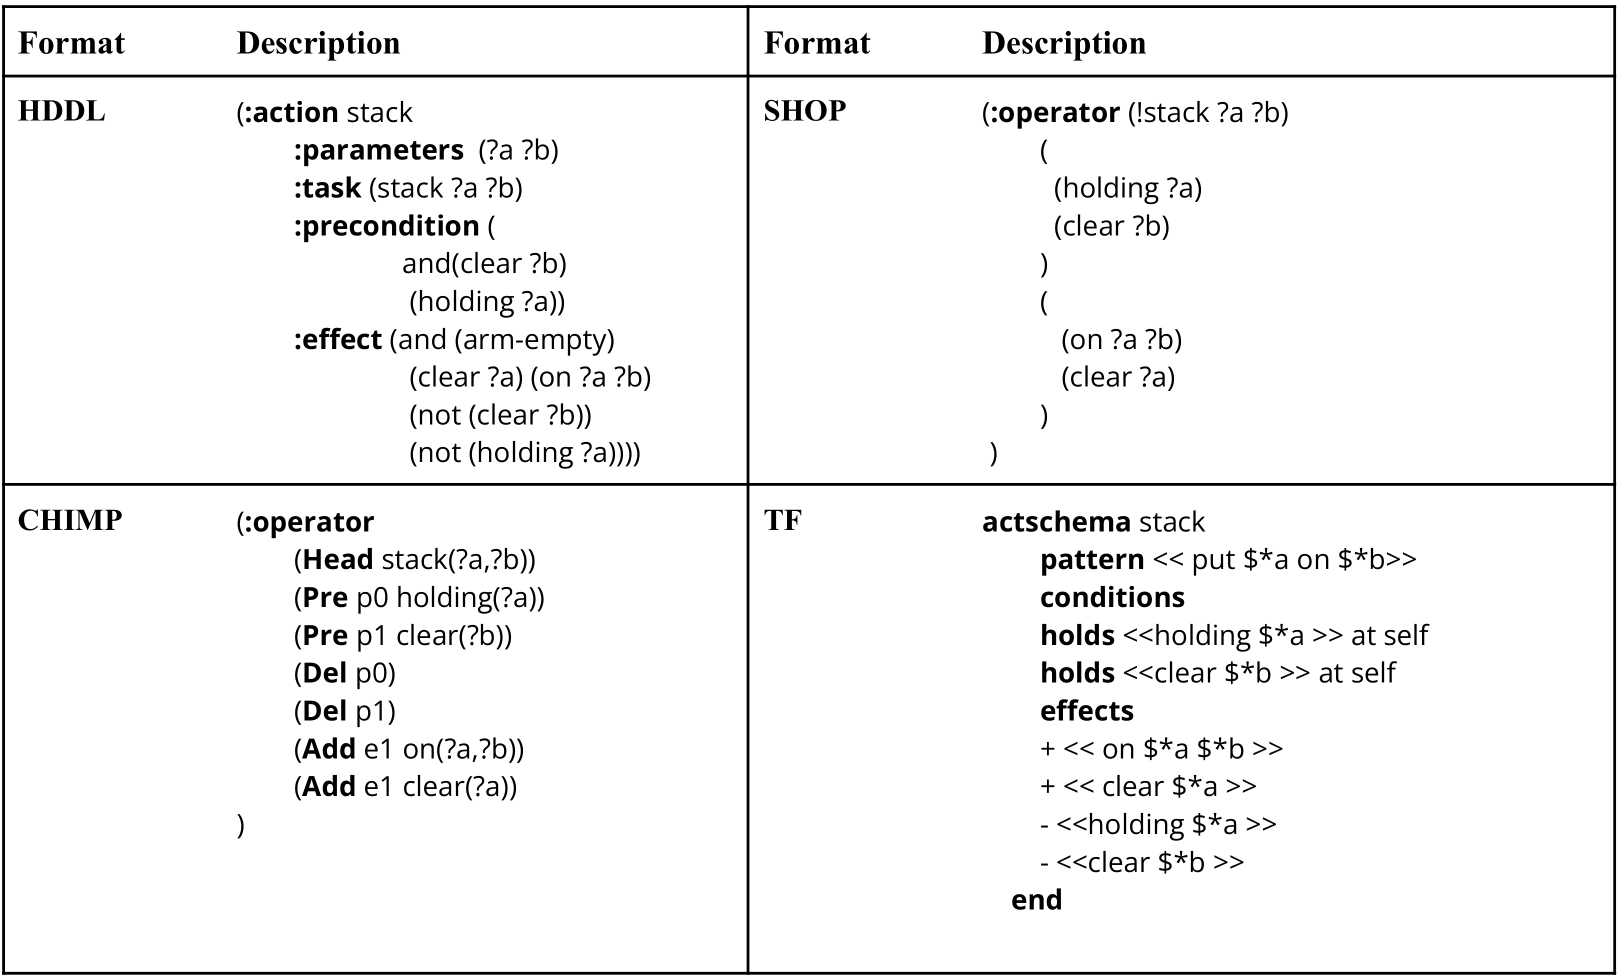
\includegraphics[width=\textwidth]{graphics/formats.png}
    \caption{The stack task from the block-world domain in different formats.}
    \label{fig:formats}
\end{figure}

There are also planners that use a programming language to describe the domain and problem rather than a specialized description language. This approach has the advantage that the planner can be directly integrated into the system using it without the need for a translation layer between the system and the planner. RAE\footnote{\url{https://github.com/patras91/rae_release}}, GTPyhop\footnote{\url{https://github.com/dananau/GTPyhop}} and FluidHTN\footnote{\url{https://github.com/ptrefall/fluid-hierarchical-task-network}} are all great examples of this approach.

\begin{Listing}
    \begin{lstlisting}[language=Python]
        def stack(s,b1,b2):
            if s.pos[b1] == 'hand' and s.clear[b2] == True:
                s.pos[b1] = b2
                s.clear[b1] = True
                s.holding['hand'] = False
                s.clear[b2] = False
                return s
    \end{lstlisting}
    \caption{The stack task from the block-world domain in GTPyhop.}
    \label{lst:StackPython}
\end{Listing}

% Utility
\section{Utility and Risk Awareness}
\label{sec:utilityAnRisk}

Classical HTN planners have several advantages over classical planners, but they lack any concept of utility. Classical HTN planners are satisfied when a solution is found, but in the real world, this is rarely sufficient. In the real world, we are typically interested in finding an optimal solution in some sense. For instance, we may only be interested in solutions that are safe, fast, or inexpensive. This section will provide an overview of the notion of utility and how it can be utilized to guide the planning process.

\subsection{Utility}
The core concept of utility revolves around modeling the outcomes of an action or situation based on a set of criteria or metrics, which allows us to rank actions or outcomes and choose the most preferable option. Mathematically, utility can be represented via a set of binary relations over a set of actions or situations $\mathbf{\Delta}$ \cite{fishburn1968utility}.

\begin{Tdef}[Preference-indifference relation $\preceq$]
    The preference-indifference relation $\preceq$ is a binary relation over a set of actions/situations $\mathbf{\Delta}$ that satisfies the following:
    $$\forall \delta_1, \delta_2 \in \Delta : \delta_1 \preceq \delta_2 \vee \delta_1 \npreceq \delta_2$$
    $\delta_1 \preceq \delta_2$ means that $\delta_1$ is not preferred to $\delta_2$.
\end{Tdef}

\begin{Tdef}[Strict preference relation $\prec$]
    The strict preference relation $\prec$ is a binary relation over a set of actions/situations $\mathbf{\Delta}$ that satisfies the following:
    $$\forall \delta_1, \delta_2 \in \Delta : \delta_1 \prec \delta_2 \Longleftrightarrow \delta_1 \preceq \delta_2 \wedge \delta_2 \npreceq \delta_1$$
    $\delta_1 \prec \delta_2$ means that $\delta_2$ is preferred to $\delta_1$.
\end{Tdef}


\begin{Tdef}[Indifference relation $\sim$]
    The indifference relation $\sim$ is a binary relation over a set of actions/situations $\mathbf{\Delta}$ that satisfies the following:
    $$\forall \delta_1, \delta_2 \in \Delta : \delta_1 \sim \delta_2 \Longleftrightarrow \delta_1 \preceq \delta_2 \wedge \delta_2 \preceq \delta_1$$
    $\delta_1 \sim \delta_2$ means that $\delta_1$ is indifferent to $\delta_2$.
\end{Tdef}

The previous binary relations form an invaluable framework that enables us to rank solutions, given that we have a model that can map any action/situation to a numeric value (utility). It is essential to recognize that utility and value do not constitute the same concept. For example, in the context of commuting to work, one can use the train or a taxi. The train would cost two dollars, whereas the taxi would cost twenty. These values do not take into consideration factors such as comfort, speed, or emissions. Concrete values such as cost and time are objective, whereas utility is quite subjective. An agent with an emphasis on comfort would give the train a lower utility score. In comparison, an agent with an emphasis on reducing emissions would give the train a higher utility score.


\subsection{Utility-based HTN planning}
One way of utilizing utility to guide an HTN planner is to assign each operator a utility score, but this is insufficient. HTN structures are intrinsically hierarchical, and the utility of a task is not necessarily identical to the utility of its subtasks. A significantly better approach is to assign a utility score to each operator, method, and compound task. The utility of a task is then the sum of its own utility and the utility of its most preferred subtask. In addition, it is essential to bear in mind that utility is extremely dynamic. Therefore, the planner must be able to recalculate the utility of each task as the planning process progresses or whenever the environment's state changes.

\begin{figure}[H]
    \centering
    \begin{tikzpicture}
        \node {$T_c$(commute\_to\_work)} [sibling distance = 6cm]
            child { 
                node{$M_1$(with\_train)} 
                child{ 
                        node{$T_c$(go\_to\_train\_station)}
                        child {
                            node{$T_p$(board\_train)}
                            child {
                                node{$T_p$(depart\_the\_train)}
                                child{
                                    node{$T_c$(walk\_the\_remaining\_distance)}
                                }
                            }
                        }
                    }
                }
            child {
                node{$M_2$(with\_taxi)}
                child{ 
                        node{$T_c$(call\_taxi)}
                        child {
                            node{$T_p$(board\_taxi)}
                            child {
                                node{$T_p$(depart\_taxi)}
                                child{
                                    node{$T_c$(walk\_the\_remaining\_distance)}
                                }
                            }
                        }
                    }
                };
    \end{tikzpicture}
    \caption{A simple HTN task network for commuting to work.}
    \label{fig:commute_to_work}
\end{figure}
Figure ~\ref{fig:commute_to_work} shows a simple HTN task network for commuting to work. This example will help us to illustrate the necessity of having a utility score for each HTN construct. If we exclusively assign utility values to the operators, there will be no way to express whether an agent prefers or dislikes using the train, for example. The compound task \qq{walk\_the\_remaining\_distance} can be reached via two distinct paths, and it would be illogical to assign it the same utility in both scenarios. The compound task \qq{commute\_to\_work} itself could have an inherently low utility value if the agent prefers to work from home.

We will refrain from providing a concrete algorithm for integrating utility into HTN planning since it is highly dependent on the search strategies implemented by the planner and because it has already been done in \cite{alnazer2019htn} \cite{georgievski2014utility} \cite{alnazer2022risk}. However, we will go over our own implementation in detail later on.

\subsection{Expected utility}
Basic utility is an effective tool for comparing solutions and ensuring that the agent always chooses the solution with the most preferable outcome. However, basic utility assumes that the world is deterministic and that each action has only one outcome, which significantly impacts its applicability in the real world, where uncertainty is a fundamental challenge.
To illustrate the limitations of basic utility, consider the scenario shown in Figure~\ref{fig:expected_utility} in which an agent is offered the choice between two actions, $\delta_1$ and $\delta_2$. There are two possible outcomes for action $\delta_1$: the agent will receive three dollars 40\% of the time, and nothing the remaining 60\% of the time. Action $\delta_2$ also has two possible outcomes: 10\% of the time, the agent will receive seven dollars, and 90\% of the time, it will receive nothing.

\begin{figure}[H]
    \centering
    \begin{tikzpicture}
        \node {} [sibling distance = 2.5cm]
            child{
                node{$\delta_1$}[sibling distance = 1.5cm]
                child{node{3} edge from parent node [left] {0.4}}
                child{node{0} edge from parent node [right] {0.6}}
            }
            child{
                node{$\delta_2$}[sibling distance = 1.5cm]
                child{node{7} edge from parent node [left] {0.1}}
                child{node{0} edge from parent node [right] {0.9}}
            };
        \end{tikzpicture}
        \caption{A simple example of hypothetical game.}
        \label{fig:expected_utility}
\end{figure}

If the agent is acting solely based on basic utility, it will always choose action $\delta_2$ since its utility value is greater, In contrast, a rational agent will virtually always choose action $\delta_1$ because it has a greater expected value:
$$ \mathbbm{E}(\delta_2) = 0.1 \times 7 + 0.9 \times 0  < \mathbbm{E}(\delta_1) = 0.4 \times 3 + 0.6 \times 0 $$

In the previous example, we assumed that the agent had based its decision on the expected value, which can lead us to the wrong conclusion that the expected value can be used to represent expected utility. However, it was clear from the early stages of research that rational agents do not always act based on expected value. As previously discussed, value is an objective concept, whereas utility is far more subjective and can be influenced by an agent's preferences, needs, and risk tolerance. Expected value fails to capture the subjective nature of utility; thus, it is not a suitable tool for representing expected utility. To further illustrate this point, we need to introduce the \textit{St. Petersburg paradox}\footnote{\url{https://en.wikipedia.org/wiki/St._Petersburg_paradox}}, which demonstrates how an agent whose only criteria for decision-making is expected value would propose a course of action that no rational agent would ever consider:

\begin{quotation}
    A hypothetical casino in St. Petersburg offers the following game to a single player:
    After paying a fixed entrance fee, a fair coin is tossed until the first head appears, which ends the game. When the game ends, the player wins $2^n$, where $n$ is the round where the first head appeared.
\end{quotation}

Now the question is, \textit{how much would a rational agent be willing to pay as an entrance fee to play this game?}

An agent using the expected value would be willing to pay an entrance fee up to the game's expected value which is infinite:
$$  \mathbbm{E} = \frac{1}{2} \cdot 2 + \frac{1}{4} \cdot 4 + \frac{1}{8} \cdot 8 + \frac{1}{16} \cdot 16 + \dots = \infty$$

which contradicts the fact that no rational agent would be willing to pay an arbitrarily large entrance fee to play this game. A better approach would be to define a utility function $\mathfrak{u}$ that reflects the agent's preferences. We can use $\mathfrak{u}$ to define the expected utility of an action $\delta$ over the probability distribution $\mathbbm{P}$ of all its possible outcomes $\Omega$.

\begin{Tdef}[Expected Utility]
    The expected utility of an action $\delta$ is the weighted sum of all possible outcomes of $\delta$:
    $$\mathbbm{E}(\delta) = \sum_{\omega} \mathbbm{P}(\omega) \cdot \mathfrak{u}(\omega)$$
\end{Tdef}

Using expected utility, we can extend our prefrence relations:
\vspace{-0.5em}
\begin{subequations}
    \begin{align*}
    \forall \delta_1, \delta_2 \in \Delta: \quad& \\
    & \delta_1 \preceq \delta_2 \Longleftrightarrow \mathbbm{E}(\delta_1) \leq \mathbbm{E}(\delta_2) \\
    & \delta_1 \prec \delta_2 \Longleftrightarrow \mathbbm{E}(\delta_1) < \mathbbm{E}(\delta_2) \\
    & \delta_1 \sim \delta_2 \Longleftrightarrow \mathbbm{E}(\delta_1) = \mathbbm{E}(\delta_2) \\
    \end{align*}
\end{subequations}

\subsection{Risk attitude}
As mentioned earlier, the utility function is a highly subjective model of the world that reflects the agent's preferences, most notably its risk tolerance. In this section, we provide a short overview of the standard risk attitude models and how the risk attitude can guide the behavior of an agent.

Sometimes rational agents are inclined to change behavior when the stacks are too high. For example, let us consider the following game, where a player has a 60\% chance of winning 100 dollars and a 40\% chance of losing 1 dollar. Conversely, some players would simply refuse to play the game because losing one dollar is too much of a risk. Some players would be willing to play the game, but they might also refuse to play if the stakes were higher. In other words, the risk attitude can be defined as the change in utility based on the ratio of potential wins to potential losses.

It is difficult to quantitatively model risk, and different fields have attempted to do so using different theories; since we cannot cover all of them here, we will explore the topic from the agent's viewpoint.

Maximizing gains or minimizing losses would be the primary goal of a naive agent. Such an agent would have an indifferent attitude toward risk (\textit{Risk neutral}). This type of agent will always choose a course of action that maximizes/minimizes its gains/losses, regardless of the risk involved.

\begin{figure}[H]
    \centering
    \begin{minipage}{.5\textwidth}
      \centering
      \begin{tikzpicture}
        \node (a){} [sibling distance = 2.5cm]
            child{
                node(b){$\delta_1$}[sibling distance = 1.5cm] 
                child{node(c){100} edge from parent[ultra thick] node [left,black] {0.7}}
                child{node(d){-40} edge from parent[solid, thin] node [right] {0.3}}
                edge from parent[ultra thick] 
            }
            child{
                node(e){$\delta_2$}[sibling distance = 1.5cm]
                child{node(f){40} edge from parent node [left] {0.1}}
                child{node(g){-10} edge from parent node [right] {0.9}}
            };
        \end{tikzpicture}
        
        \textit{Gain maximizing agent}
    \end{minipage}%
    \begin{minipage}{.5\textwidth}
      \centering
      \begin{tikzpicture}
        \node (a){} [sibling distance = 2.5cm]
            child{
                node (b){$\delta_1$}[sibling distance = 1.5cm]
                child{node(c){100} edge from parent node [left] {0.7}}
                child{node(d){-40} edge from parent node [right] {0.3}}
            }
            child{
                node(e){$\delta_2$}[sibling distance = 1.5cm]
                child{node(f){40} edge from parent[solid, thin] node [left] {0.1}}
                child{node(g){-10} edge from parent node [right] {0.9}}
                edge from parent[ultra thick] 
            };
        \end{tikzpicture}
        
        \textit{Loss minimizing agent}
    \end{minipage}
    \caption{Risk-neutral agents' decision-making}
    \label{fig:risk-neutral}
\end{figure}

Figure \ref{fig:risk-neutral} shows two agents that are risk neutral. The first agent is gain-maximizing, and the second agent is loss-minimizing. The gain-maximizing agent will always choose $\delta_1$ because it has a higher potential gain of 100. Whereas the loss-minimizing agent will always choose $\delta_2$ because it has a lower potential loss, even though the probability of losing 10 is much higher than the probability of losing 40, the agent will still choose $\delta_2$. Risk-neutral agents will always have a linear utility function. This means that the utility of an outcome is proportional to the outcome itself. More rational agents tend to be more sensitive to risk, especially when dealing with high-stakes situations. In general, rational agents show a tendency to avoid high risks when the payoff is insufficient to compensate for them, and they usually prefer an action course with a lower payoff and a higher probability of success. In addition, rational agents sometimes accept to bear small losses in order to avoid situations where there is a low probability of suffering a very large loss. This type of agent is called \textit{Risk-Averse}.

\begin{figure}[H]
    \centering
    \begin{minipage}{.5\textwidth}
      \centering
      \begin{tikzpicture}
        \node {} [sibling distance = 2.5cm]
            child{
                node{$\delta_1$}[sibling distance = 1.5cm] 
                child{node{100} edge from parent node [left,black] {0.6}}
                child{node{-100} edge from parent node [right] {0.4}}
            }
            child{
                node{$\delta_2$}[sibling distance = 1.5cm]
                child{node{40} edge from parent node [left] {0.7}}
                child{node{-10} edge from parent[ultra thick] node [right] {0.3}}
                edge from parent[ultra thick] 
            };
        \end{tikzpicture}
        
        \textit{Lower potential payoff and loss}
    \end{minipage}%
    \begin{minipage}{.5\textwidth}
      \centering
       \begin{tikzpicture}
        \node {} [sibling distance = 2.5cm]
            child{
                node{$\delta_1$}[sibling distance = 1.5cm] 
                child{node{-5} edge from parent node [left,black] {1}}
                edge from parent[ultra thick] 
            }
            child{
                node{$\delta_2$}[sibling distance = 1.5cm]
                child{node{0} edge from parent node [left] {0.99}}
                child{node{-1000} edge from parent node [right] {0.01}}
            };
        \end{tikzpicture}
        
        \textit{Small loss over an unlikely very big loss}
    \end{minipage}
    \caption{Risk-averse agents' decision-making}
    \label{fig:risk-averse}
\end{figure}

Two distinct situations are shown in Figure \ref{fig:risk-averse} to illustrate how an agent with a risk-averse attitude will always choose the action that involves the lowest risk. The utility function of a risk-averse agent is concave, with low risk outcomes having a bigger utility score. Some agents are inherently more risk loving (\textit{Risk-Seeking}). They will be more willing to take risks in order to achieve a higher payoff, even if it involves a higher risk. The utility function of a risk-seeking agent is convex, with high profitability outcomes having a bigger utility score. Figure \ref{fig:risk-seeking} shows how a risk-seeking agent will behave in the same previously shown situations.

\begin{figure}[H]
    \centering
    \begin{minipage}{.5\textwidth}
      \centering
      \begin{tikzpicture}
        \node {} [sibling distance = 2.5cm]
            child{
                node{$\delta_1$}[sibling distance = 1.5cm] 
                child{node{100} edge from parent node [left,black] {0.6}}
                child{node{-100} edge from parent[thin] node [right] {0.4}}
                edge from parent[ultra thick] 
            }
            child{
                node{$\delta_2$}[sibling distance = 1.5cm]
                child{node{40} edge from parent node [left] {0.7}}
                child{node{-10} edge from parent node [right] {0.3}}
            };
        \end{tikzpicture}
        
       \textit{Higher potential payoff and loss}
    \end{minipage}%
    \begin{minipage}{.5\textwidth}
      \centering
       \begin{tikzpicture}
        \node {} [sibling distance = 2.5cm]
            child{
                node{$\delta_1$}[sibling distance = 1.5cm] 
                child{node{-5} edge from parent node [left,black] {1}}
            }
            child{
                node{$\delta_2$}[sibling distance = 1.5cm]
                child{node{0} edge from parent node [left] {0.99}}
                child{node{-100} edge from parent[thin] node [right] {0.01}}
                edge from parent[ultra thick] 
            };
        \end{tikzpicture}
        
         \textit{Accepts the risk}
    \end{minipage}
    \caption{Risk-seeking agents' decision-making}
    \label{fig:risk-seeking}
\end{figure}

Typically, an agent's preferences and risk tolerance will be dynamic, changing based on a broad range of factors such as current wealth, type of risk, and previous experiences. These factors make it hard to model the agent's preferences in one mathematical construct; however, \cite{alnazer2022risk} proposes some risk-based utility functions. Figure \ref{fig:risk-based-utility} shows how the utility function of an agent might look based on their risk attitude.




\begin{figure}[H]
    \centering
    \begin{minipage}{.3\textwidth}
      \centering
      \begin{tikzpicture}[scale = 0.5]
        \begin{axis}[
            legend style={at={(1,0.2)},anchor=north east,draw=white},
            axis lines=middle,
            axis line style = thick,
            ticks=none,
            xlabel={Gain},
            ylabel={Utility},
            xlabel style={at={(ticklabel* cs:1)},anchor=north west},
            ylabel style={at={(ticklabel* cs:1)},anchor=north east},
            xmin=0, xmax=10,
            ymin=0, ymax=10,
          ]
          \addplot [
            domain=0:9,
            color=black,
          ]
          {x};
          \addlegendentry{risk neutral}
        \end{axis}
      \end{tikzpicture}
    \end{minipage}
    \hspace{1em}
    \begin{minipage}{.3\textwidth}
      \centering
      \begin{tikzpicture}[scale = 0.5]
        \begin{axis}[
            legend style={at={(1,0.2)},anchor=north east,draw=white},
            axis lines=middle,
            axis line style = thick,
            ticks=none,
            xlabel={Gain},
            ylabel={Utility},
            xlabel style={at={(ticklabel* cs:1)},anchor=north west},
            ylabel style={at={(ticklabel* cs:1)},anchor=north east},
            xmin=0, xmax=100,
            ymin=0, ymax=2,
          ]
  
          \addplot [
            domain=1:80,
            color=black,
            samples=100
          ]
          {log10(x)};
          \addlegendentry{risk averse}
        \end{axis}
      \end{tikzpicture}
    \end{minipage}
    \hspace{1em}
    \begin{minipage}{.3\textwidth}
      \centering
      \begin{tikzpicture}[scale = 0.5]
        \begin{axis}[
            legend style={at={(1,0.2)},anchor=north east,draw=white},
            axis lines=middle,
            axis line style = thick,
            ticks=none,
            xlabel={Gain},
            ylabel={Utility},
            xlabel style={at={(ticklabel* cs:1)},anchor=north west},
            ylabel style={at={(ticklabel* cs:1)},anchor=north east},
            xmin=0, xmax=10,
            ymin=0, ymax=100,
          ]
          \addplot [
            domain=-2:9,
            color=black,
            samples=100
          ]
          {x^2};
          \addlegendentry{risk-seeking}
        \end{axis}
      \end{tikzpicture}
    \end{minipage}
    \caption{Different risk-based utility functions}
    \label{fig:risk-based-utility}
\end{figure}

At the end of this section, we would like to point out that although it has been shown \cite{kahneman2013prospect} that the expected utility theory fails as a descriptive theory due to its inability to predict human behavior in some situations successfully, it is a very suitable normative theory that can be used to guide the decision-making process of rational agents, especially when combined with a good dynamic utility function.

\subsection{Risk attitude and HTN planning}
Our model of utility-based HTN planning can be easily extended to enable agents to make decisions based on their risk attitude by having a utility function that takes into account the risk involved in the decision. One benefit that we have is that we are not bound to one mathematical construct; we can have multiple utility functions corresponding to different risk attitudes, and we can switch between them, choosing the function that better suits the agent's current situation. This allows our agents to have a more flexible and dynamic attitude toward risk. We can also utilize the rule-based nature of HTN to create a set of rules that can override the current risk attitude of an agent in some situations where we believe the agent would be better off with a more or less risk-sensitive attitude. Let us consider the following scenario where we have a stock-trading agent: The agent has a hand-crafted utility function with an overall risk-averse attitude that is based on a plethora of financial and economic factors. However, it would be beneficial for the agent to have a set of rules in place that can override its risk tolerance in real time to react to sudden changes in the market. Such rules should not only be used to change the agent's attitude toward risk; they can also be used to directly interfere and change the evaluation of a given action to be more or less risky. Going back to our previous example, shorting a stock\footnote{\url{https://en.wikipedia.org/wiki/Short_(finance)}} is usually a big risk that should be avoided. However, if Warren Buffet\footnote{\url{https://en.wikipedia.org/wiki/Warren_Buffett}} is shorting stock X with a large sum of money, the action of shorting that stock should no longer be seen as risky.

Lastly, we would like to note that it is beneficial to utilize the concept of risk attitude in HTN agents even when the concept of utility is not modeled since it enables us to group actions and guide the decision-making process using one dynamic switch.

\begin{Listing}
    \begin{lstlisting}[language=HDDL]
        (define (domain Little_Red_Riding_Hood)
            ...
            (:task get-to :parameters (?l - location ?a - riskAttitude))
            ...
            (:method stay-on-path
                :parameters (?l - location ?a - riskAttitude)
                :task (get-to ?l)
                :precondition(isRiskAverse ?a)
                ...
            )
            (:method wander-into-the-woods
                :parameters (?l - location ?a - riskAttitude)
                :task (get-to ?l ?a - riskAttitude)
                :precondition(isRiskSeeking ?a)
                ...
            )
        )
    \end{lstlisting}
    \caption{Example of using risk attitude without utility}
    \label{lst:risk-without-utility}
\end{Listing}

Listing \ref{lst:risk-without-utility} shows how we can use risk attitude without utility. In this example, we have one compound task \textbf{get-to}, that can be achieved using one of two methods \textbf{stay-on-path} or \textbf{wander-into-the-woods}. The agent will choose between these methods based on its risk attitude. Integrating risk based decision-making in this way is quite simple and it can greatly impact the behavior of an agent in a dynamic environment.

%%%%%%%%%%%%%%%%%%%%%%%%%%%%%%%%%%%%%%%%%%%%%%%%%%%%%%%%%%%%%%%%%%%%%%%%%%%%%%
%
% Main content ends here
%
%%%%%%%%%%%%%%%%%%%%%%%%%%%%%%%%%%%%%%%%%%%%%%%%%%%%%%%%%%%%%%%%%%%%%%%%%%%%%%


\chapter{Related Work}

\chapter{Conclusion and Outlook}

\section*{Outlook}

\printbibliography

All links were last followed on March 17, 2018.

\appendix

\pagestyle{empty}
\renewcommand*{\chapterpagestyle}{empty}
\Versicherung
\end{document}
